\documentclass{beamer}
%\usepackage{default}
\usepackage{amsmath}
\usepackage{graphicx}
\usepackage{adjustbox}  % Allows for fitting tables into slide
%\usepackage{hyperref}
\usepackage{threeparttable}
\usepackage{caption}
%\usepackage{subcaption}
\usepackage{natbib}
\usepackage{adjustbox}
\usepackage{subcaption}
\usepackage{hyperref}
\hypersetup{
	colorlinks = true,
	linkcolor=.,
	citecolor= {cyan}
}
\usepackage{comment}

\usepackage{bbm}

%\usetheme{AnnArbor}
%\usetheme{Antibes}
%\usetheme{Bergen}
%\usetheme{Berkeley}
%\usetheme{Berlin}
%\usetheme{Boadilla}
%\usetheme{boxes}
\usetheme{CambridgeUS}
%\usetheme{Copenhagen}
%\usetheme{Darmstadt}
%\usetheme{default}
%\usetheme{Frankfurt}
%\usetheme{Goettingen}
%\usetheme{Hannover}
%\usetheme{Ilmenau}
%\usetheme{JuanLesPins}
%\usetheme{Luebeck}
%\usetheme{Madrid}
%\usetheme{Malmoe}
%\usetheme{Marburg}
%\usetheme{Montpellier}
%\usetheme{PaloAlto}
%\usetheme{Pittsburgh}
%\usetheme{Rochester}
%\usetheme{Singapore}
%\usetheme{Szeged}
%\usetheme{Warsaw}

% colortheme to choose one 

%\usecolortheme{beaver}
%\usecolortheme{crane}
%\usecolortheme{default}
\usecolortheme{dolphin}
%\usecolortheme{seagull}
%\usecolortheme{seahorse}
%\usecolortheme{whale}


% fond theme to choose one 
%\usefonttheme{structuresmallcapsserif}
%\usefonttheme{structureitalicserif}
%\usefonttheme{structurebold}
\usefonttheme{serif}
%\usefonttheme{professionalfonts}
%\usefonttheme{default}

\title{Perceived Income Risks}


% A subtitle is optional and this may be deleted

\author{Tao Wang \\ Johns Hopkins University}
% - Give the names in the same order as the appear in the paper.
% - Use the \inst{?} command only if the authors have different
%   affiliation.

\date{\today \\
	Macro/Finance Brownbag Seminar}
% - Either use conference name or its abbreviation.
% - Not really informative to the audience, more for people (including
%   yourself) who are reading the slides online

% This is only inserted into the PDF information catalog. Can be left
% out. 

% If you have a file called "university-logo-filename.xxx", where xxx
% is a graphic format that can be processed by latex or pdflatex,
% resp., then you can add a logo as follows:

% \pgfdeclareimage[height=0.5cm]{university-logo}{university-logo-filename}
% \logo{\pgfuseimage{university-logo}}

% Delete this, if you do not want the table of contents to pop up at
% the beginning of each subsection:


% Abstract Workhorse incomplete-market macro models typically assume that agents have a perfect understanding of the size and nature of income risks that econometricians estimate from past income data. This paper examines if risk perceptions from a representative density survey align with these assumptions. I found that people have reasonable clues about income risks in that the differences in risk perceptions can be partly explained by intra-group differences in income volatility. But there remains a large degree of intrinsic heterogeneity. There is also strong evidence for state-dependence, past dependence, and tail risks. Risk perceptions countercyclically react to recent realizations and past experiences of macro labor markets.  My ongoing work incorporates such survey-implied heterogeneity in risk perceptions and state dependence into a life-cycle/incomplete market model and explores its implications for consumption/saving decisions and wealth inequality of the economy. 


%\AtBeginSubsection[]
%{
%	\begin{frame}<beamer>{Outline}
%	\tableofcontents[ currentsection,
%	sectionstyle=show,
%	subsectionstyle=show]
%\end{frame}
%}

\begin{document}
	

\begin{frame}
	\titlepage
\end{frame}
\begin{frame}{Outline}
	\tableofcontents
	% You might wish to add the option [pausesections]
\end{frame}


\section{Motivation}


\begin{frame}{Motivation}
	\begin{itemize}
		\item Risks matter for \textcolor{orange}{individual decisions}
		\begin{itemize}
			\item precautionary saving 
			\item stock market participation
			\item portfolio choice 
		\end{itemize} 
		%%Not just expectation of income but also \textcolor{blue}{high moments} such as income risks matter for consumption/portfolio decisions, i.e. precautionary motives, stock market investment, etc. 
		\item Risks matter for \textcolor{orange}{macroeconomic outcomes}
		\begin{itemize}
			\item since idiosyncratic risks are not perfectly insured 
			\begin{itemize}
				\item $\rightarrow$ income/wealth inequality 
				\item $\rightarrow$ heterogeneous $MPC$s
				\item $\rightarrow$ distributional channel of macroeconomic policies 
				\item $\rightarrow$ business cycle fluctuations
			\end{itemize}
		\end{itemize}  %%\textcolor{blue}{Uninsurance} of idiosyncratic risks make it matter in macroeconomics, i,e. the important assumption by the HANK literature
	\item Income risks are central inputs of any incomplete-market model   
		\item My question:  \textcolor{red}{perceptions} $\approx$ \textcolor{blue}{estimates}  $\approx$  ``the truth''?  %%It is unclear if perceptions consistent with econometricians' estimates of income risks from cross-sectional inequality and the those used in structural models   What enter in people's calculation are \textcolor{blue}{perceived} risks 
		%%People make  their decisions based on there \textit{their} perceptions
	\end{itemize}
\end{frame}


\begin{frame}{Some macro facts}
	\begin{itemize}
	\item Wealth inequality and heterogeneity in $MPC$s
	\begin{itemize}
		\item a standard incomplete market model generates \textcolor{orange}{insufficient inequality seen in the data}
		\item unless additional features such as \textcolor{orange}{preference heterogeneity} or \textcolor{orange}{costly adjustment} are introduced 
	\end{itemize}
\item Liquid assets holdings 
\begin{itemize}
	\item \textcolor{orange}{too few} in data compared to a standard one-asset incomplete market model 
\end{itemize}
\item ``Excessive sensitivity'' to unanticipated transitory shocks 
\begin{itemize}
	\item  \textcolor{orange}{high $MPC$s} seen in the data than $PIH$ model prediction 
\end{itemize}
	\end{itemize}
\end{frame}


\begin{frame}{Preview of the findings}
	%% the first part mostly empirical.  The second part is the theory. My talk will be primarily about the first part. This is what I have achieved so far. But also I feel there are many interesting facts per se. More importantly, this empirical regularity can better discipline and guide my modeling work. 
	\begin{enumerate}
		\item \textbf{Empirics:} subjective risk profiles from a density survey
		\begin{itemize}
			\item \textcolor{blue}{Heterogeneity}: sizable difference across/within groups
			\item \textcolor{blue}{Superior information}: on average lower than standard parameterizations used by economists 
			\item \textcolor{blue}{State-dependence}: negative correlation with recent/past labor market conditions 
				\item \textcolor{blue}{Extrapolation}:  correlated with negative labor outcomes
			\item \textcolor{blue}{History-dependence}: positive correlation with experienced volatility/unemployment 
			%\item \textcolor{blue}{Asymmetry}: presence of tail risks
			\item \textcolor{blue}{Decisions}: spending plans react to risk perceptions
			
			% sensible but imperfect risks 

		
			%\item differ systematically by \textcolor{blue}{income, age, generation,  and education}
			%\item affect  \textcolor{blue}{planned spendings} 
			%\item non-normality, i.e half of population have
			%\textcolor{blue}{non-zero skewness}
		\end{itemize}
\pause
		\item \textbf{Model}: 
		\begin{itemize}
			\item a survey-informed \textcolor{red}{subjective} OLG / incomplete-market GE model 
\begin{itemize}
	\item Lower PR $\rightarrow$ lower savings
	\item State-dependence/extrapolation $\rightarrow$ higher savings
	\item Heterogeneity in PR $\rightarrow$ wealth inequality 
\end{itemize}
		\end{itemize} 
	\end{enumerate}
\end{frame}


\begin{frame}{Literature}
	\begin{itemize}
		\item income risks and partial insurance :{\scriptsize\cite{gottschalk1994growth}, \cite{carroll1997nature}, \cite{meghir2004income}, \cite{storesletten2004cyclical}, \cite{blundell_consumption_2008},
		\cite{moffitt2002trends},  \cite{guvenen2014nature},  \cite{arellano2017earnings}, \cite{bloom2018great}}
		\item subjective/probabilistic survey of beliefs: {\scriptsize\cite{manski_measuring_2004}, \cite{delavande2011measuring}, \cite{manski_survey_2018},  \cite{bertrand_people_2001}, \cite{armantier_overview_2017}}
		\item incomplete market macro: {\scriptsize\cite{bewley1976permanent}, 
		 \cite{aiyagari1994uninsured},
		\cite{huggett1996wealth}, \cite{krusell1998income}, \cite{heathcote2009quantitative},  \cite{carroll2017distribution}, \cite{krueger2016macroeconomics},  \cite{bayer2019precautionary}}
		%\item ``insurance or information'':  \cite{kaufmann_disentangling_2009},  \cite{meghir2011earnings}, \cite{pistaferri_superior_2001}, New York Fed Blog (2019),  \cite{flavin_excess_1988}
		\item consumption/saving under incomplete information/imperfect perception:  {\scriptsize\cite{pischke1995individual}, \cite{wang2004precautionary}, \cite{rozsypal_overpersistence_2017}, \cite{carroll_sticky_2018}, \cite{lian2019imperfect}}
		%\item macroeconomic expectation formation: \cite{coibion2012can}, \cite{fuhrer2018intrinsic}, etc
	
	\end{itemize}
\end{frame}


\section{Theoretical framework}

\begin{frame}{Log income process}
	\begin{equation*}
		\begin{split}
			\underbrace{y_{i,c,t}}_{\text{idiosyncratic log earning}} = \underbrace{z_{i,c,t}}_{\text{predictable component}}  + \underbrace{e_{i,c,t}}_{\text{stochastic component}}
		\end{split} 
	\end{equation*}
	
	\begin{itemize}
		\item individual \(i\) at time \(t\) 
		\item group $c$: share income process/risks $\sigma^2_{c,t}$
		\begin{itemize}
			\item i.e. education/year of birth/gender/age
		\end{itemize}
		\item $e_{i,c,t}$: to be specified later
	\end{itemize}
\end{frame}

\begin{frame}{Perceived risks (PR)}
	\begin{itemize}
		\item Income growth 
		\begin{equation*}
			\begin{split}
				\Delta y_{i,c,t+1} & =\Delta z_{i,c,t+1} +\Delta e_{i,c,t+1} 
			\end{split}
		\end{equation*}
		\item \textcolor{red}{To the agent: \textbf{expected volatility} under FIRE}
		\begin{equation*}
			\begin{split}
				Var^*_{i,c,t}(\Delta y_{i,c,t+1}) & =\sigma^2_{c,t+1|t}
			\end{split}
		\end{equation*}
		\item \textcolor{blue}{To econometricians: \textbf{volatility} } 
		\begin{equation*}
			\begin{split}
			Var^c(\Delta \hat e_{i,c,t+1})     = \hat\sigma^2_{c,t}+ \hat\sigma^2_{c,t+1} - 2Cov^c(\hat e_{i,c,t},\hat e_{i,c,t+1})
			%Var^c(\hat e_{i,c,t+1})
			\end{split}
		\end{equation*}
%	\item \textcolor{blue}{To econometricians: \textbf{inequality} } 
%		\begin{equation*}
%		\begin{split}
%		Var^c( \hat e_{i,c,t+1}) = \sigma^2_{c,t+1}
%		\end{split}
%	\end{equation*}
	\end{itemize}	
%% therefore, I can examine how gross volatility estimated for each cohort is positively correlated with perceived risk from the data. 
%% nice things about using gross volatility 
%% not sensitive the stochastic nature of e
%% not sensitive to the frequency of the data from PSID being annual or biennial 
\end{frame}

\begin{comment}
\begin{frame}{Predictions from FIRE}

	\begin{itemize}
		\item  PR equal within groups with identical  risks 
		\begin{itemize}
			\item \textcolor{blue}{Question}: do similar people perceive similar degree of risks?
		\end{itemize}
		\item PR $\uparrow$ with income volatility
		\begin{itemize}
			\item \textcolor{blue}{Question}: do groups with higher volatility/inequality perceive higher risks?
			%\item the correlation depends on the time series nature of $e_{i,c,t}$ and $\sigma^2_{c}$
		\end{itemize}
		% $$Cov(Var^c(\hat e_{i,c,t}),Var^*_{i,c,t}(\Delta y_{i,c,t+1}))\approx 1$$
		\item PR independent from the income realization under state-independent risks
		\begin{itemize}
			\item \textcolor{blue}{Question} correlated with past/recent outcomes?
			%\item unless $\sigma^2_{e}$ is state dependent 
		\end{itemize} 
	\end{itemize} 
\end{frame}

\begin{frame}{Robustness to alternative considerations}
	
	\begin{itemize}
		\item superior information/unobserved heterogeneity
		    \begin{itemize}
			\item higher income volatility/inequality due to omitted variable
		    \end{itemize}
		\item measurement error in PR
		\begin{itemize}
			\item lower correlation but still positive
		\end{itemize}
		\item time aggregation
	\begin{itemize}
		\item higher frequency of income than observed series 
		%\item it matters once we assume time series property of $e$
	\end{itemize}
		\item time-varying/stochastic risks 
		\begin{itemize}
			\item a concern if realizations and perceptions not overlapping in time
			\item time-invariant risks for now: $\sigma^2_{c,t}=\sigma^2_{c} \quad \forall t$
		\end{itemize}
	\end{itemize} 
\end{frame}
\end{comment}

\section{Empirical evidence}

\begin{frame}{Data and sample}
	\begin{itemize}
		\item Density survey: SCE
		\begin{itemize}
			\item 2013M6-2020M4   (monthly)
			\item 1300 households 
			\item 12-month panel 
		\end{itemize}
\item Income panel: PSID 
\begin{itemize}
	\item 1970-1996 (annual), 1997-2017 (biennial) 
	\item approximately 5000 males/females 
	\item variable: wage/earning of household heads 
	\item stay in the sample for 11+ years
	\item CPI adjusted 
	\item age 20-59 
\end{itemize}
\item Income Panel: SIPP
\begin{itemize}
	\item 2014M1-2019M12 (monthly)
	\item earning from the primary job 
	\item 900-2700 respondents 
		\item CPI adjusted 
	\item age 20-59

\end{itemize}
\end{itemize}
\end{frame}


%%%%%%%%%%%%%%%%%%%%%%%%%%%%%%%%%%%%%%%%%%%%%%%%%%%%%%%%%%%
%% need to change the time stamp!!!!!!!!!!!!!!!
%%%%%%%%%%%%%%%%%%%%%%%%%%%%%%%%%%%%%%%%%%%%%%%%%%%%%

\begin{frame}{Survey question}
	\begin{itemize}
		\item Individual-specific bin-based forecast on $\Delta y_{i,t+1}$
		\begin{itemize}
			\item earning growth of the same job/position/hours
				\item exl. endogenous labor supply changes/promotion/demotion/separation 
				%\item Can be converted into the unconditional risk using perceived unemployment risk ( same-job-hour risk is just a lower bound).  %% I did not do the adjustment. I use same-job-hour income growth throughout my analysis.
		\end{itemize} 
		\item  Measurement of PR: 
		\begin{itemize}
			%\item expected growth, $\text{exp}_{i,t} = E_{i,t} (\Delta Y_{i,t+12})$
			\item variance: \textcolor{blue}{$\overline {Var}_{i,t}(\Delta y_{i,t+1})$} 
			% \item iqr: $\overline {iqr}_{i,t}(\Delta y_{i,t+12})$ 
			%\item skewness: $\overline {Skew}_{i,t}(\Delta y_{i,t+1})$
		\end{itemize}
		%\item nominal and real income growth 
		%\begin{itemize}
			%\item $\text{rexp}_{i,t} =E_{i,t}(\Delta y^r_{i,t+1}) =E_i(\Delta y_{i,t+1}^n) - E_{i,t+1}(\pi_{t+1})$
		%	\item $\overline{rvar}_{i,t}=\overline {var}_{i,t}(\Delta y_{i,t+1}^n) +  \overline {var}_{i,t}(\pi_{t+1})$
\item density estimation following \cite{engelberg_comparing_2009}			
\item restricted to attentive/high numeracy score sample
\item adjusted into real terms using inflation uncertainty 
\end{itemize}
\end{frame}


\begin{frame}{An illustration of the density forecast estimation}
	\begin{figure}
		\centering
		\label{fig: dens_est_illutration}
			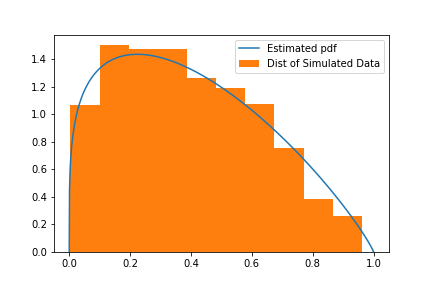
\includegraphics[width=0.6\textwidth]{figures/dens_est_illutration.png}
	\end{figure}

\begin{itemize}
	\item  case 1. 3+ intervals with positive probs, to be fitted with a generalized beta distribution
	\item case 2. exactly 2 adjacent intervals with positive probs, to be fitted with a triangle distribution 
	\item case 3. one interval only, to be fitted with a uniform distribution
\end{itemize}

\end{frame}




\subsection{Cross-sectional patterns}


%%% the purpose of examining cross-sectional distribution are twofold. First, since there is not much work that has been showing these basic facts. I think it is important to be aware of new facts. Second, for those of you who are still a little doubtful about the survey data, it helps us assure the surveyed data shows some patterns that are intuitive and consistent.  

%\begin{frame}{Cross-sectional of income growth expectation}
%	\begin{figure}
%		\centering
%		\label{incexp_hist}
%		\begin{subfigure}[b]{0.45\textwidth}
%			\centering
%			\caption{expected growth of nominal}
%			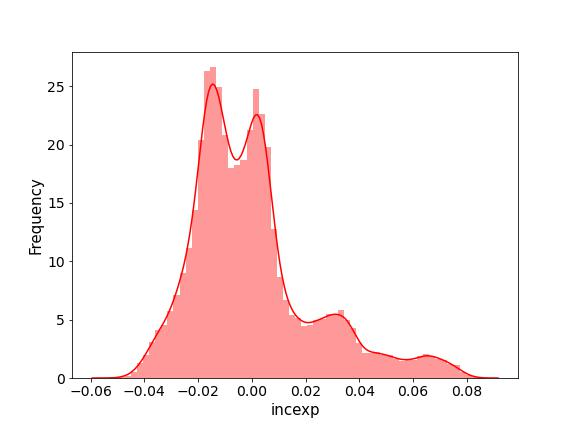
\includegraphics[width=\textwidth]{figures/hist_incexp}
%		\end{subfigure}
%		\begin{subfigure}[b]{0.45\textwidth}
%			\centering
%			\caption{expected growth of real}
%			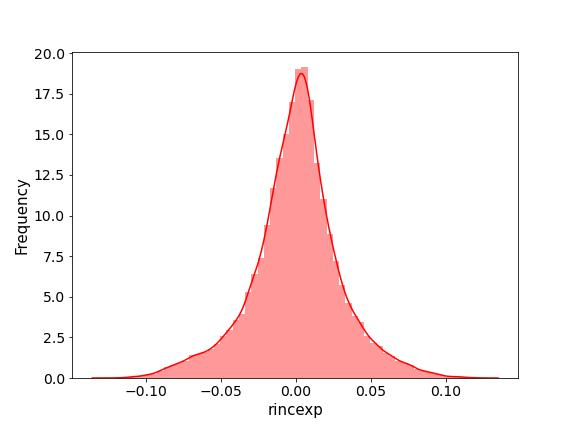
\includegraphics[width=\textwidth]{figures/hist_rincexp}
%		\end{subfigure}
%	\end{figure}
%	\begin{itemize}
%		\item nominal income: right-skewed and mostly positive   
%		\item real income: symmetric around zero  
%	\end{itemize}
%\end{frame}

\begin{frame}{Within-group dispersion in perceived income risks}
	\begin{figure}
		\centering
		\label{rincstd_hist}
%			\begin{subfigure}[b]{0.45\textwidth} 
%			\centering
%			\caption{income risks (nominal)}
%		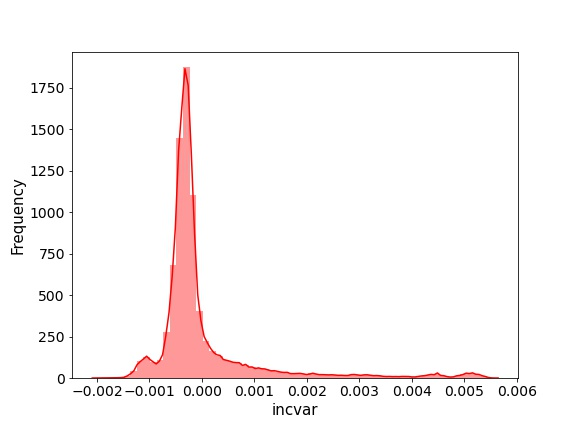
\includegraphics[width=\textwidth]{figures/hist_incvar.jpg}
%		\end{subfigure}
	%	\begin{subfigure}[b]{0.45\textwidth}
%		\centering
%		\caption{income risks}
		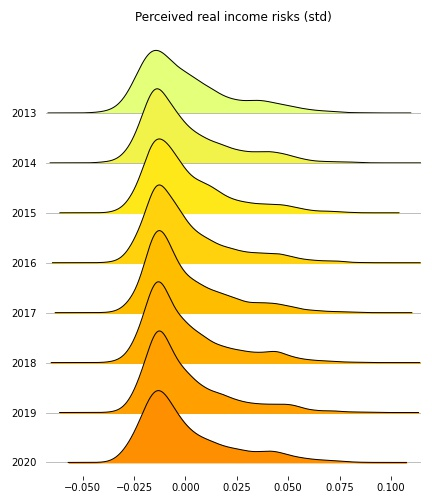
\includegraphics[width=0.4\textwidth]{figures/joy_rincstd.jpg}
%	\end{subfigure}
	\end{figure}
	\begin{itemize}
		\item  residuals controlling for observables $+$ time FE ($R^2=0.07$) 
		\item average PR:  $3.5\%$ in std; 10/90 IQR: $5.2\%$ in std \quad \hyperlink{appendix:incstd}{\beamerbutton{nominal}}  \quad
		 \hyperlink{appendix:incskew}{\beamerbutton{skewness}}    
% \item just a lower bound: before adjustment of unemployment risk 
	\end{itemize}
\end{frame}



\begin{frame}{By \textbf{age}/gender/education}
	\label{age_compare}
	\begin{figure}[ht]
		%\caption{Perceived Risk} 
		\label{compare_by_age_gender_educ}
		\centering
		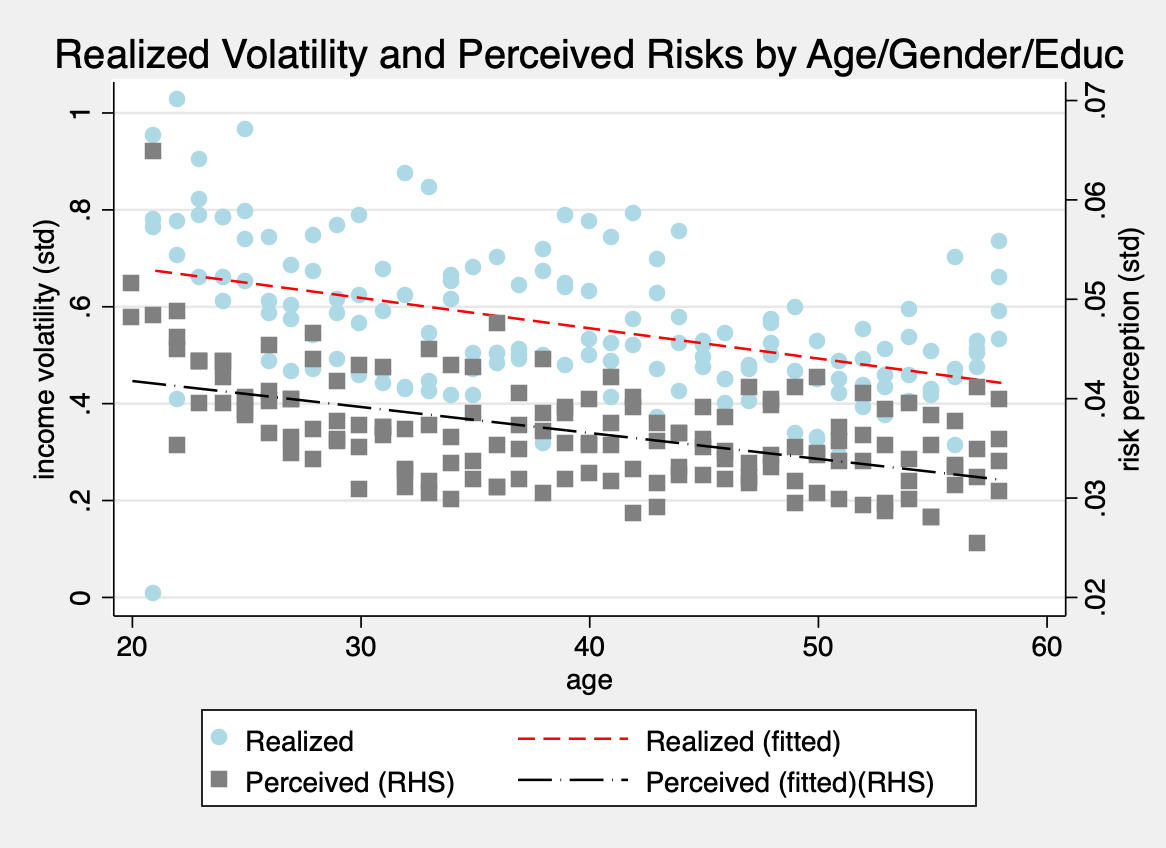
\includegraphics[width=0.60\textwidth]{figures/real_log_wage_shk_gr_by_age_edu_gender_compare.png}
	\end{figure}
	\begin{itemize}
		\item e.g. a male high school graduate aged 30   \hyperlink{appendix:age_gender_educ_compare_figure}{\beamerbutton{inequality}} \quad \hyperlink{appendix:age_compare_figure}{\beamerbutton{by age}}  
		\quad  \hyperlink{appendix:age_educ_compare_figure}{\beamerbutton{by age/education}}  
		\quad  \hyperlink{appendix: compare_by_cohort}{\beamerbutton{by 5-yr of birth/education/gender}}  
		\item consistent with  \cite{moffitt2002trends}, \cite{sabelhaus2010great}
	\end{itemize}
	%\hyperlink{monthly_decomposition_compare}{\beamerbutton{Back}} 
\end{frame}

\begin{comment}
\begin{frame}{Perceived risks by annual earning}
	\begin{figure}
		\centering
		\label{boxplot_hhinc}
		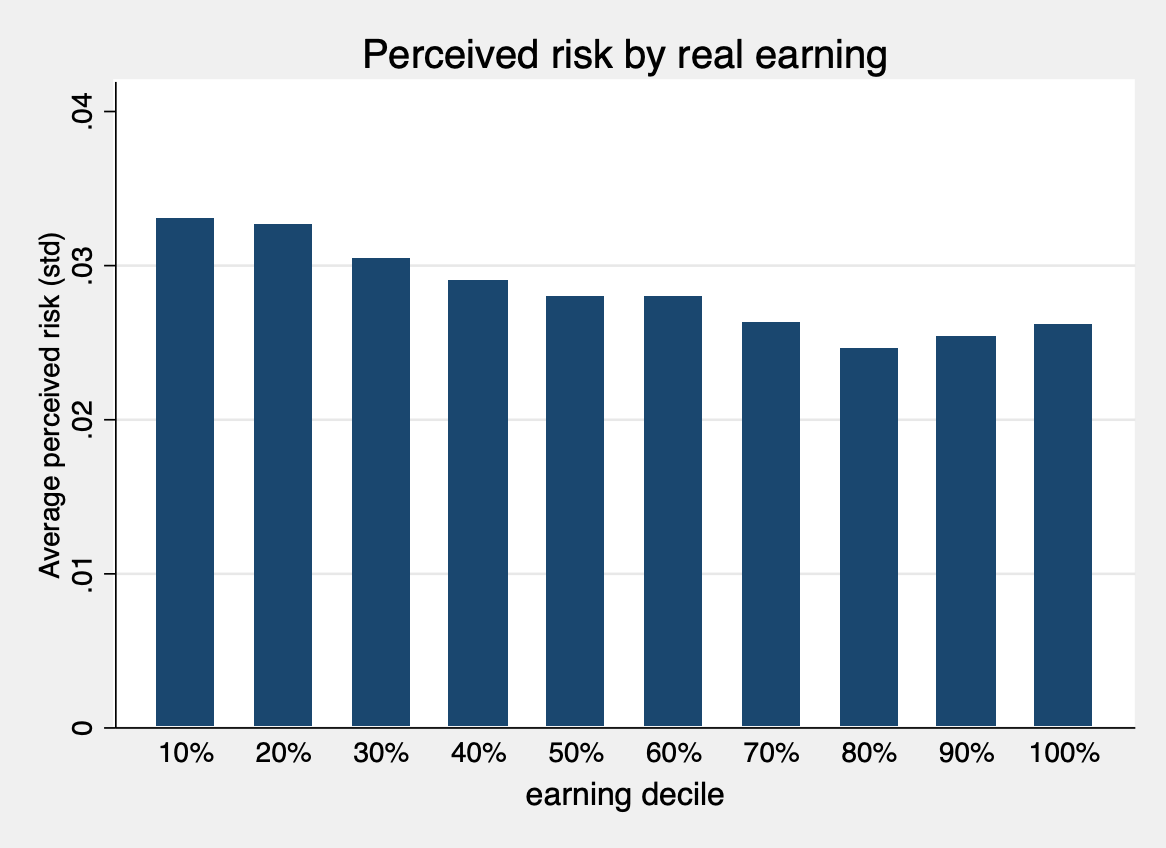
\includegraphics[width=0.7\textwidth]{figures/boxplot_rvar_earning}
	\end{figure}
	%\begin{itemize}
	%\item Similar to the pattern of earning growth dispersion conditional on income in \cite{bloom2018great}. 
	%\end{itemize}
 \end{frame}



\begin{frame}{Appendix: PR by age/gender/education}
	\begin{figure}[ht]
		%\caption{Perceived Risk} 
		\label{appendix:age_gender_educ_compare_figure}
		\centering
		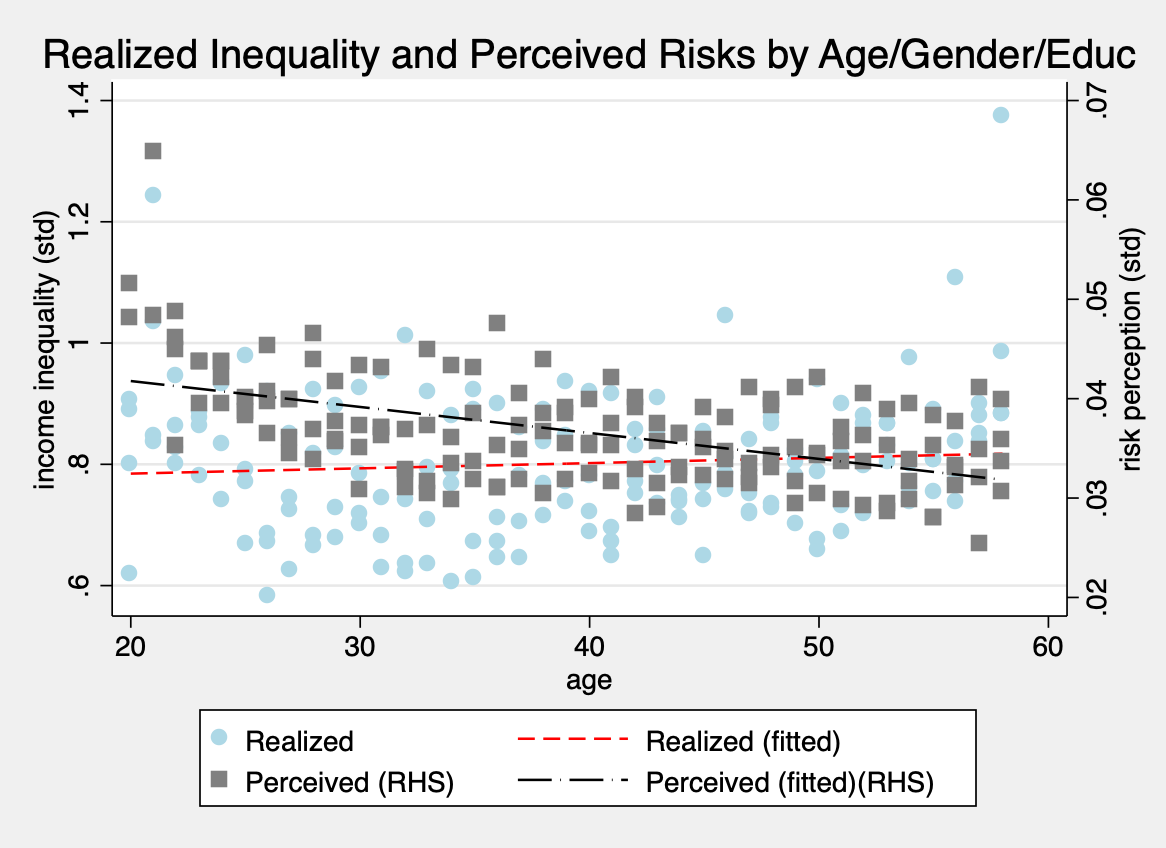
\includegraphics[width=0.7\textwidth]{figures/real_log_wage_shk_by_age_edu_gender_compare.png}
	\end{figure}
	\begin{itemize}
		\item age /gender/education  \quad  \hyperlink{age_compare}{\beamerbutton{Back}} 
		%	\item in line with existing findings, for instance  
		%	\cite{bloom2018great}. 
	\end{itemize}
\end{frame}



\begin{frame}{By \textbf{5-yr of birth/age}}
	\label{cohort_age_compare}
	\begin{figure}[ht]
		%\caption{Perceived Risk} 
		\label{compare_by_cohort_age}
		\centering
		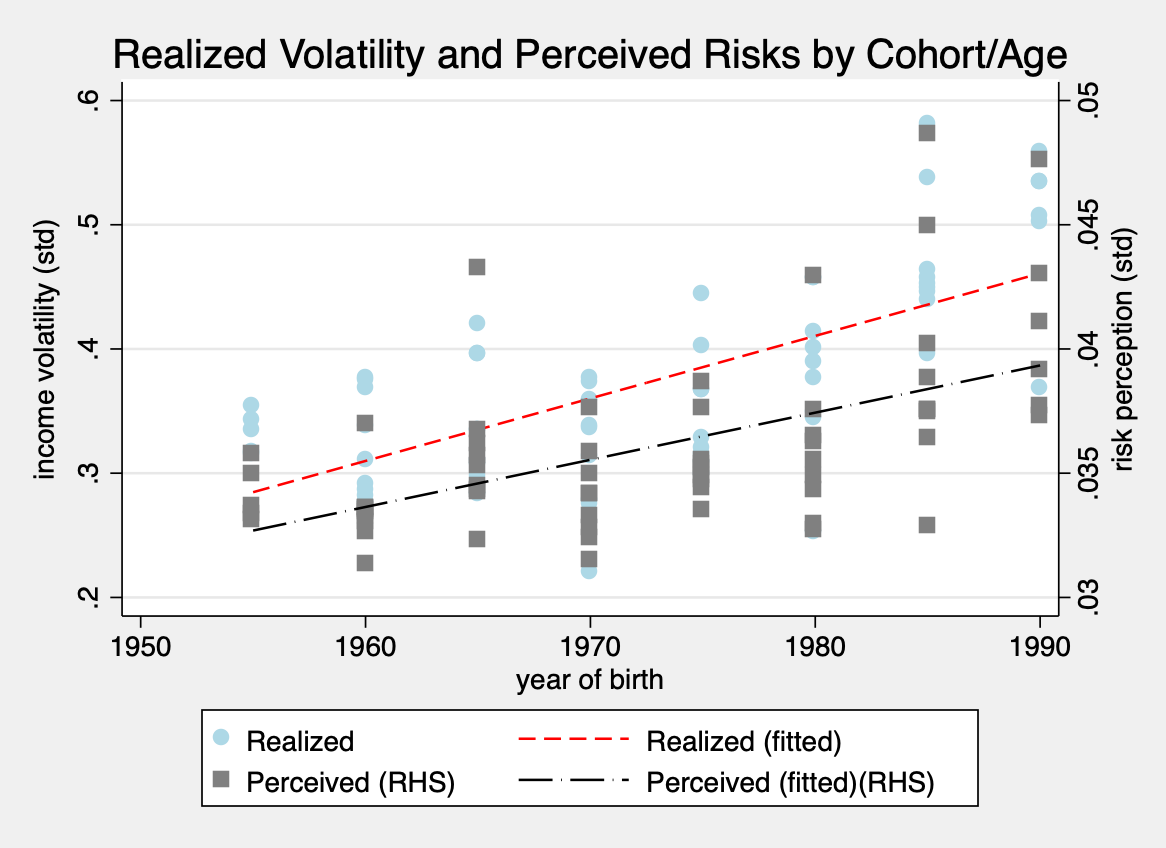
\includegraphics[width=0.65\textwidth]{figures/real_log_wage_shk_gr_by_byear_age_compare.png}
		%	\begin{subfigure}[b]{0.46\textwidth}
		%			\caption{skewness}
		%			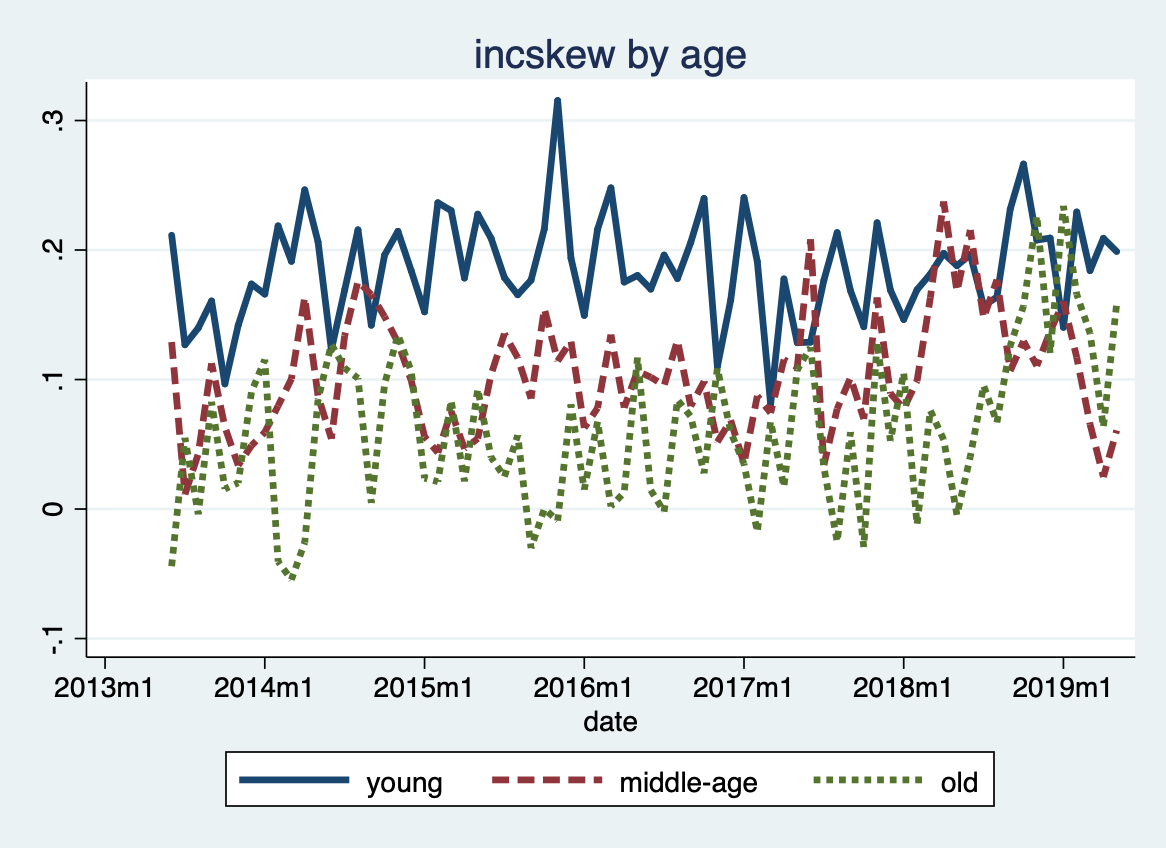
\includegraphics[width=\textwidth, height = 0.33\textheight]{figures/ts_incskew_age_g_mean.png}
		%	\end{subfigure}
	\end{figure}
	\begin{itemize}
		\item e.g. born between 1985-1990 at age 25
		\item only possible for post-2013 sample 
			\quad \hyperlink{appendix:cohort_age_compare}{\beamerbutton{inequality}}     
	\end{itemize}
\end{frame}

\end{comment}


\subsection{Permanent  versus transitory risks}


\begin{frame}{Time series structure of income shocks}

\begin{equation*}
	\begin{split}
& e_{i,c,t} = \underbrace{log (p_{i,c,t})}_{\text{permanent}} + \underbrace{log(\theta_{i,c,t})}_{\text{ transitory}} \\
& log (p_{i,c,t+1}) = log(p_{i,c,t}) + log (\psi_{i,c,t+1}) \\
& log (\psi_{i,c,t}) \sim N(\frac{-\sigma^2_{c,t,\psi}}{2},\sigma^2_{c,t,\psi}) \\
 & log (\theta_{i,c,t}) \sim N(\frac{-\sigma^2_{c,t,\theta}}{2},\sigma^2_{c,t,\theta}) \\
\end{split} 
	\end{equation*}


%\begin{itemize}
%	\item Different approaches of estimation: 
%	\begin{itemize}
%		\item approximation: \cite{moffitt2002trends}
%		\item variance/covariance matching: \cite{carroll1997nature}, \cite{meghir2004income},  \cite{blundell_consumption_2008}
%		\item continuous time: immune to time aggregation: \cite{crawley_search_2019} 
%	\end{itemize}
%\end{itemize}
\end{frame}




\begin{frame}{Permanent versus transitory risks (from monthly earning data)}
	\label{monthly_decomposition_compare}
	\begin{figure}[ht]
		\centering
		\begin{subfigure}[b]{0.32\textwidth}
			\caption{permanent}
			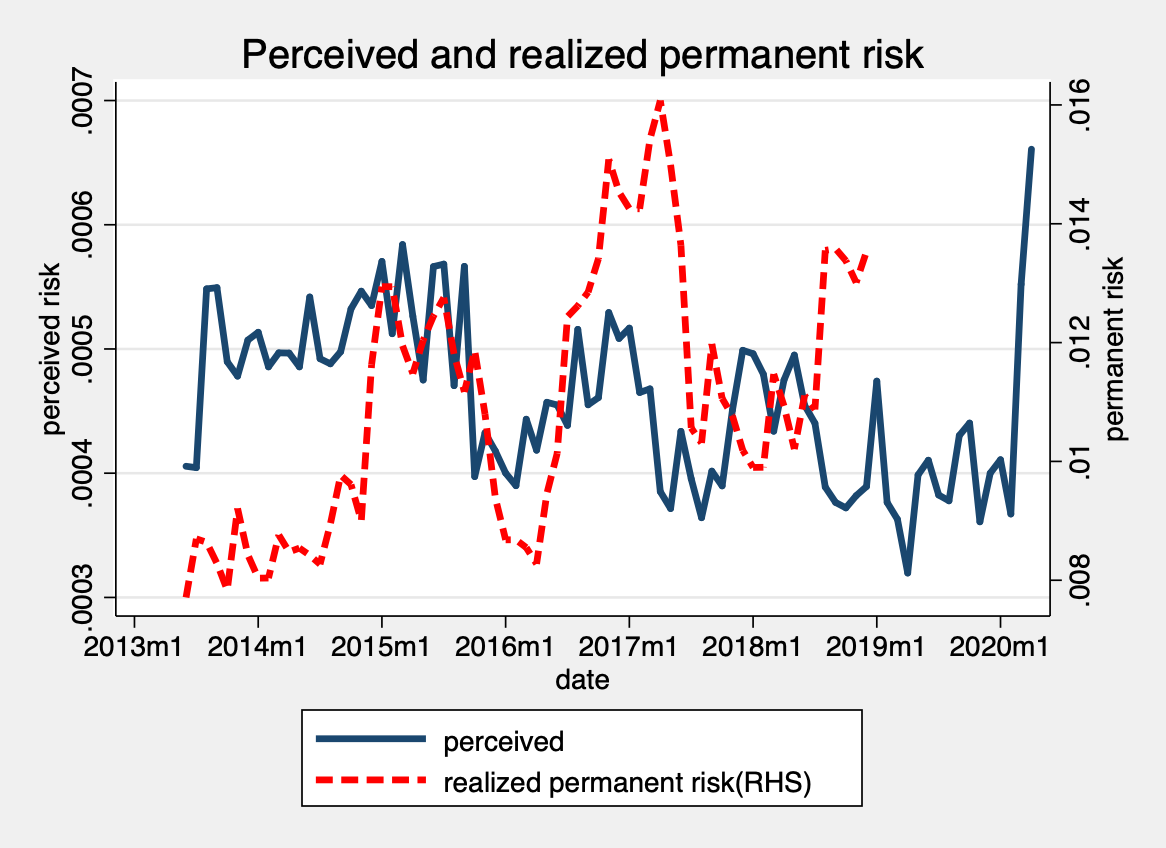
\includegraphics[width=\textwidth]{figures/real_permanent_compare.png}
		\end{subfigure}
		\begin{subfigure}[b]{0.32\textwidth}
			\caption{transitory}
			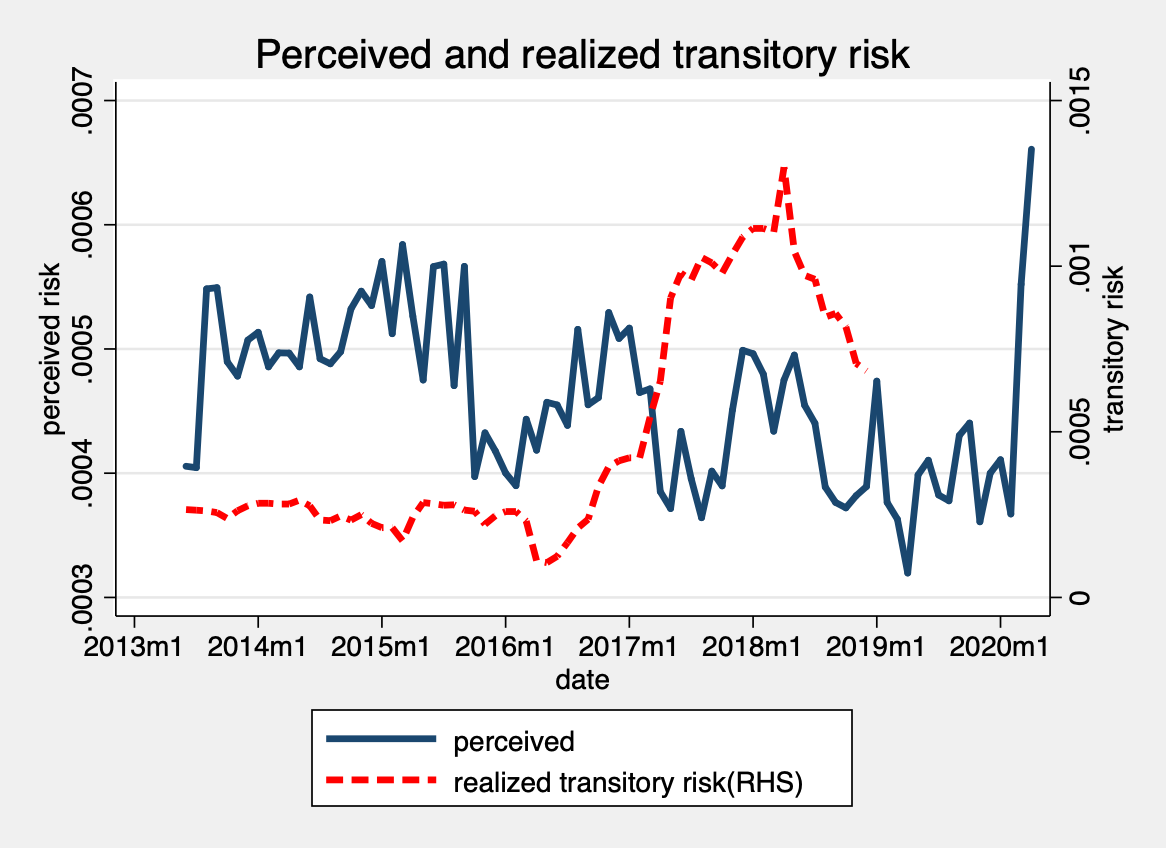
\includegraphics[width=\textwidth]{figures/real_transitory_compare.png}
		\end{subfigure} 
		\begin{subfigure}[b]{0.32\textwidth}
		\caption{volatility}
		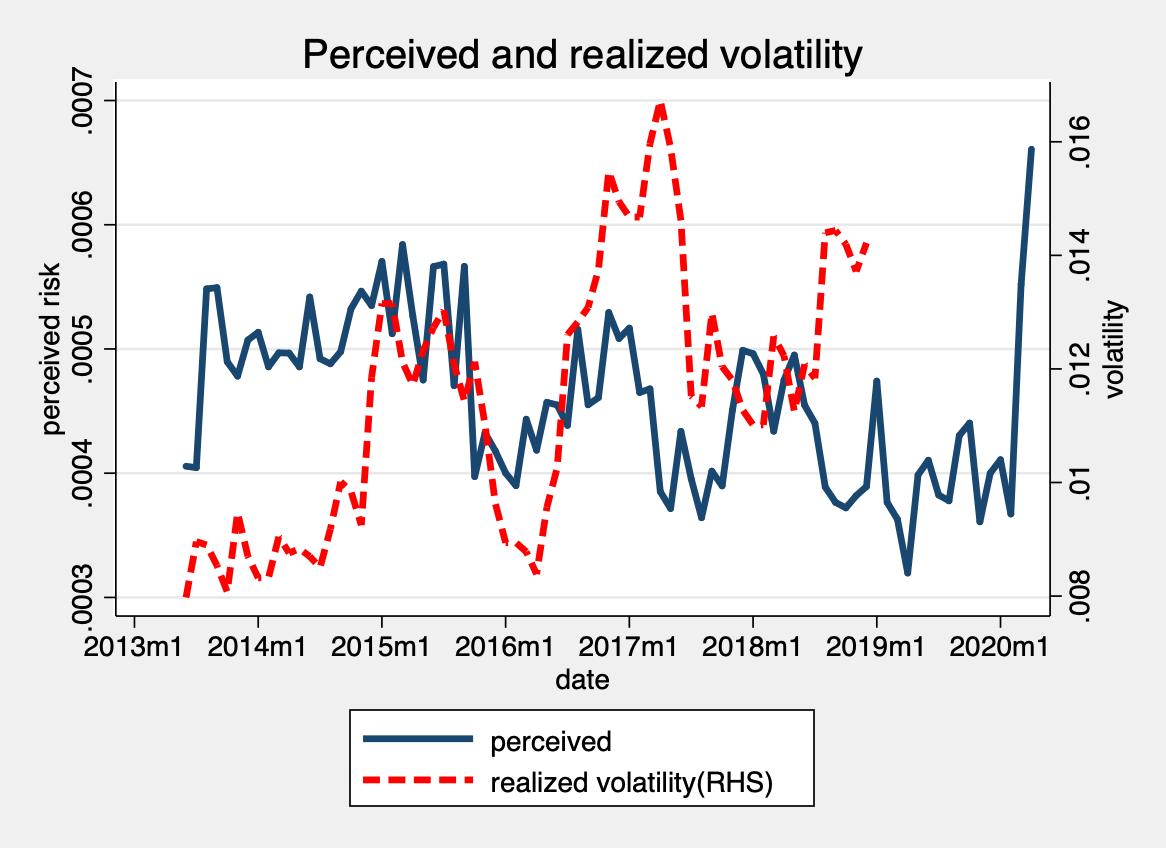
\includegraphics[width=\textwidth]{figures/real_volatility_compare.png}
	\end{subfigure} 
	\end{figure}
	\begin{itemize}
		\item i.e. one-year-ahead perceived risk at 2014m1 v.s. realized risk over the same period
		\item monthly wage rate: earning per hour of work
		\item estimated monthly risks aggregated into annual frequency 
	\end{itemize}
\hyperlink{appendix:monthly_inequality_vol}{\beamerbutton{More details}} 
\hyperlink{appendix:monthly_decomposition_compare_psid}{\beamerbutton{PSID}} 
\end{frame}



\begin{frame}{Perceptions versus economists' estimates}
	
	
	\begin{table}
		\centering
		%\caption{Estimated realized income risk and perceptions}
		\label{risk_compare}
		\adjustbox{max height=0.5\textheight, max width=\textwidth}{ 
			\begin{tabular}{llllll}
				\hline 
				\hline 
				& \textcolor{red}{PerceivedRisk} & PerceivedRisk(median) & \textcolor{blue}{RealizedGroupVolatility} & RealizedPRisk & RealizedTRisk \\
				\hline 
				full sample (100\%)        & 0.029         & 0.021                 & 0.090                   & 0.101         & 0.016       \\
				\hline 
				gender               &               &                       &                         &               &              \\
					\hline 
				
				1 (50\%)             & 0.030         & 0.022                 & 0.091                   & 0.102         & 0.016        \\
				2 (49\%)             & 0.028         & 0.022                 & 0.089                   & 0.101         & 0.016        \\
				\hline 
				
				education       &               &                       &                         &               &              \\
				\hline 
				HS dropout (0\%)     & 0.036         & 0.022                 & 0.051                   & 0.100         & 0.016        \\
				HS graduate (42\%)   & 0.030         & 0.022                 & 0.085                   & 0.101         & 0.016        \\
				College/above (56\%) & 0.028         & 0.021                 & 0.094                   & 0.101         & 0.016        \\

				\hline 
				
				5-year age           &               &                       &                         &               &              \\
					\hline 
				20 (2\%)             & 0.037         & 0.031                 & 0.072                   & 0.102         & 0.015        \\
				25 (12\%)            & 0.032         & 0.027                 & 0.115                   & 0.102         & 0.016        \\
				30 (12\%)            & 0.030         & 0.023                 & 0.091                   & 0.101         & 0.016        \\
				35 (13\%)            & 0.029         & 0.021                 & 0.098                   & 0.101         & 0.016        \\
				40 (13\%)            & 0.028         & 0.020                 & 0.084                   & 0.101         & 0.016        \\
				45 (14\%)            & 0.028         & 0.020                 & 0.065                   & 0.101         & 0.016        \\
				50 (15\%)            & 0.027         & 0.019                 & 0.078                   & 0.101         & 0.016        \\
				55 (15\%)            & 0.027         & 0.018                 & 0.105                   & 0.100         & 0.016        \\
				\hline 
			\end{tabular}
		}
	\end{table}
\end{frame}


\subsection{Perceived risks and macroeconomic history}

%% since income risks may difer over time or stochastic,  so the level of risks are not comparable directly between two non-overlapping periods. % therefore, we can treat the income volatility in the past as experiences and examine if it affects risk perceptions. Here we differ from the earlier exercise in that we do not assume the risks are cohort specific. Instead, we just assume the information set, namely the experienced volatility and inequality are different.

% we find the experienced volatility is not correlated with risk perceptions over the past. But experienced inequality is positively correlated with the risk perceptions. 
% furthermore, the average economy has negative impacts on the risk perceptions as well. 


\begin{frame}{Experienced income volatility and perceived risks}
	\begin{figure}
		\centering 
		\label{experience_var_var_var}
		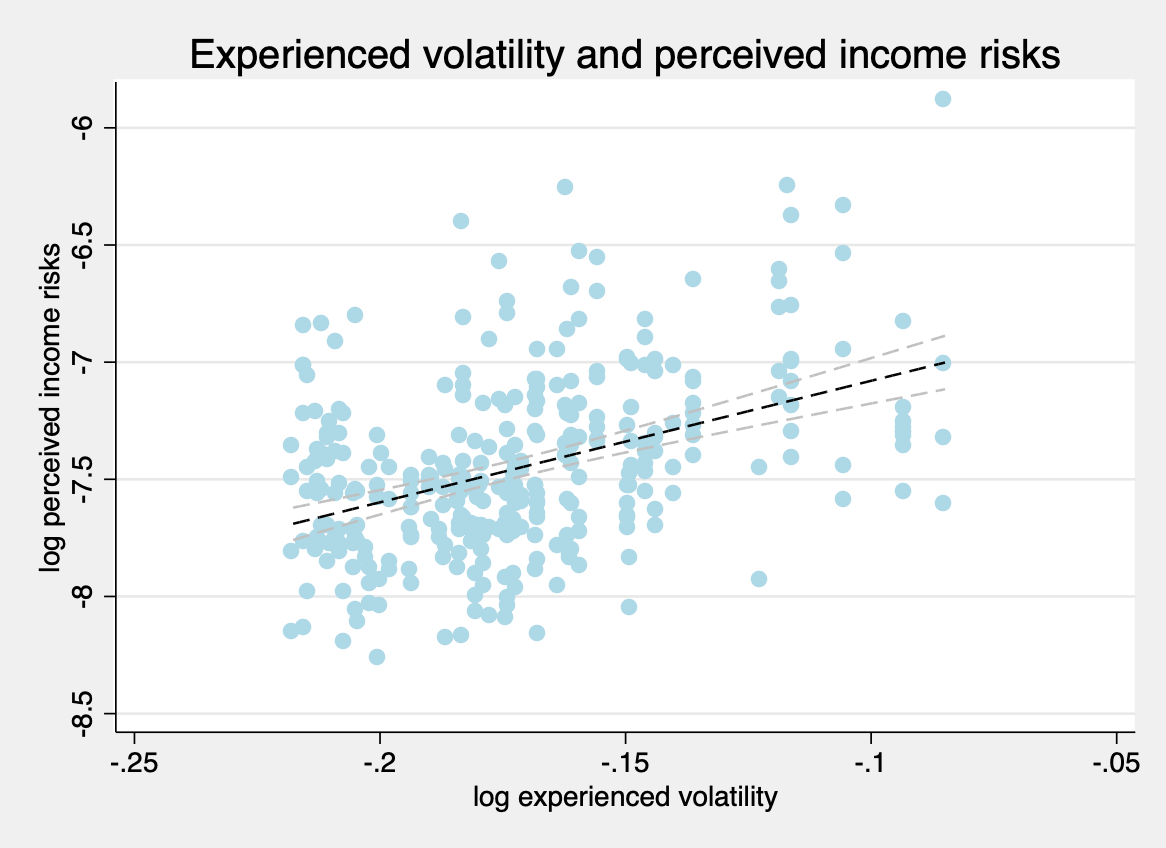
\includegraphics[width=0.6\textwidth]{figures/experience_var_var_data.png}
	\end{figure}
	\begin{itemize}
		\item income volatility conditional on macroeconomic history \cite{storesletten2004cyclical}
		\item e.g. the experience by a 25-year old till 2015 is between 1990-2015
	\end{itemize}
\end{frame}

\begin{frame}{Experienced labor market and perceived risks}
		\begin{figure}
				\centering 
				\label{experience_ue_var}
				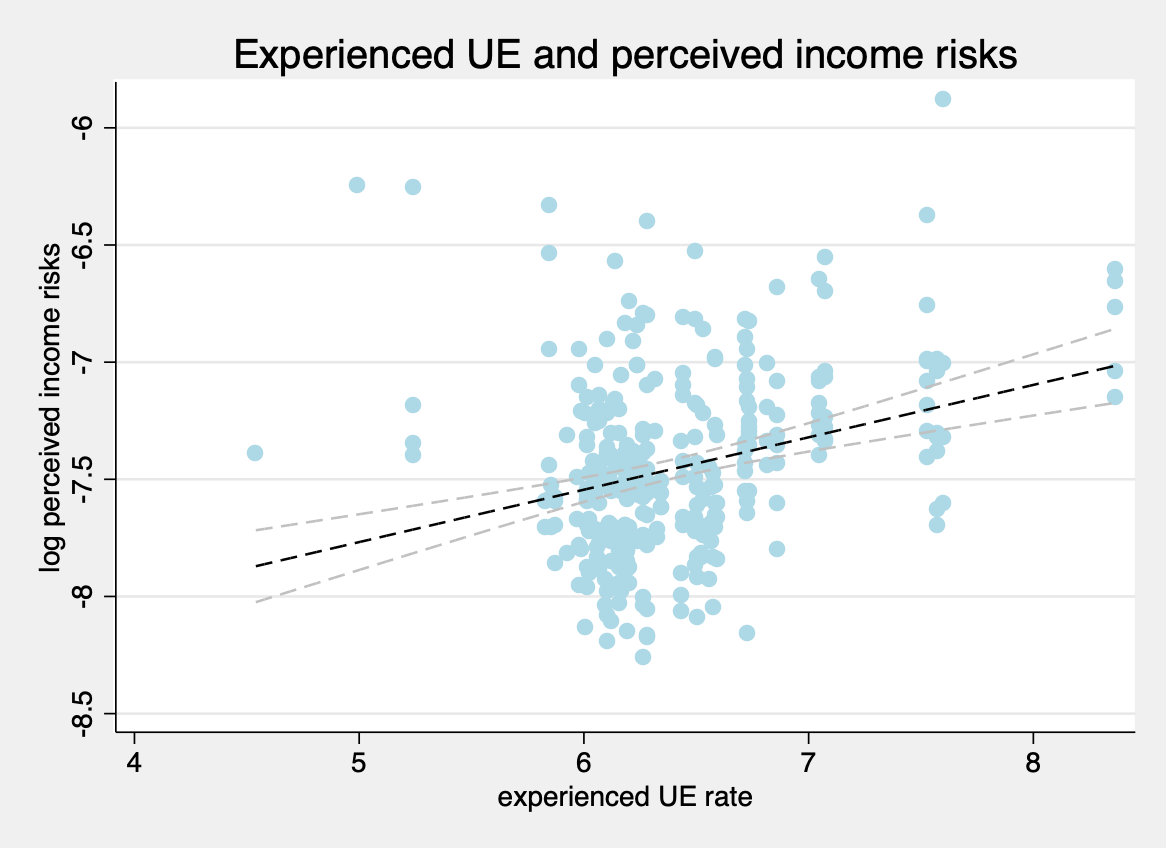
\includegraphics[width=0.6\textwidth]{figures/experience_ue_var_data.png}
			\end{figure}
	\begin{itemize}
		\item e.g. experienced UE by a 25-year old in 2015 is between UE over 1990-2015

	\end{itemize}
\end{frame}


\subsection{Extrapolation of recent experience}

\begin{frame}{Extrapolation from \textcolor{blue}{individual} experiences}
	
	\begin{itemize}
		\item higher experienced volatility $\rightarrow$ higher PR
		\item recent unemployment experience $\rightarrow$ higher PR
	\end{itemize}
	\begin{table}
		\centering
		\label{extrapolation}
		\adjustbox{max height=0.5\textheight, max width=\textwidth}{ 
			\begin{tabular}{lllllllllll}
				\hline 
				& (1)       & (2)       & (3)       & (4)       & (5)        & (6)        & (7)        & (8)        & (9)        & (10)       \\
				\hline 
				income shock squared                  & 0.0225*** & 0.0222*** & 0.0217*** & 0.0207*** & 0.000773   & 0.00205*** & 0.000566   & 0.00183*** & 0.000614   & 0.00184*** \\
				& (0.00562) & (0.00570) & (0.00562) & (0.00564) & (0.000743) & (0.000516) & (0.000744) & (0.000515) & (0.000745) & (0.000516) \\
				&           &           &           &           &            &            &            &            &            &            \\
				recently unemployed                   &           &           &           & 0.511*    & 0.228***   & 0.0895***  &            &            &            &            \\
				&           &           &           & (0.260)   & (0.0330)   & (0.0200)   &            &            &            &            \\
				&           &           &           &           &            &            &            &            &            &            \\
				unemployed since m-8&           &           &           &           &            &            & 0.161***   & 0.0783***  &            &            \\
				&           &           &           &           &            &            & (0.0207)   & (0.0121)   &            &            \\
				&           &           &           &           &            &            &            &            &            &            \\
				unemployed since y-1&           &           &           &           &            &            &            &            & 0.138***   & 0.0701***  \\
				&           &           &           &           &            &            &            &            & (0.0193)   & (0.0113)   \\
				Observations                          & 3662      & 3662      & 3662      & 3662      & 3701       & 1871       & 3701       & 1871       & 3701       & 1871       \\
				R-squared                             & 0.004     & 0.013     & 0.016     & 0.017     & 0.015      & 0.030      & 0.019      & 0.041      & 0.016      & 0.039      \\
				\hline 
			\end{tabular}
		}
	\end{table}
\end{frame}


\subsection{Countercyclical perceived risks}


\begin{frame}{Perceived risks and recent (past) wage growth}
\label{tsMean3mvrvar_he}
	\begin{itemize}
		\item $\overline{\text{var}_{t}} $: average perceived risk across individuals
		\item  $log(\text{wage}_t) - log(\text{wage}_{t-1/4})$: quarterly growth in average hourly wage
	\end{itemize}
	\begin{figure}
		\centering
		\label{ts_var}
		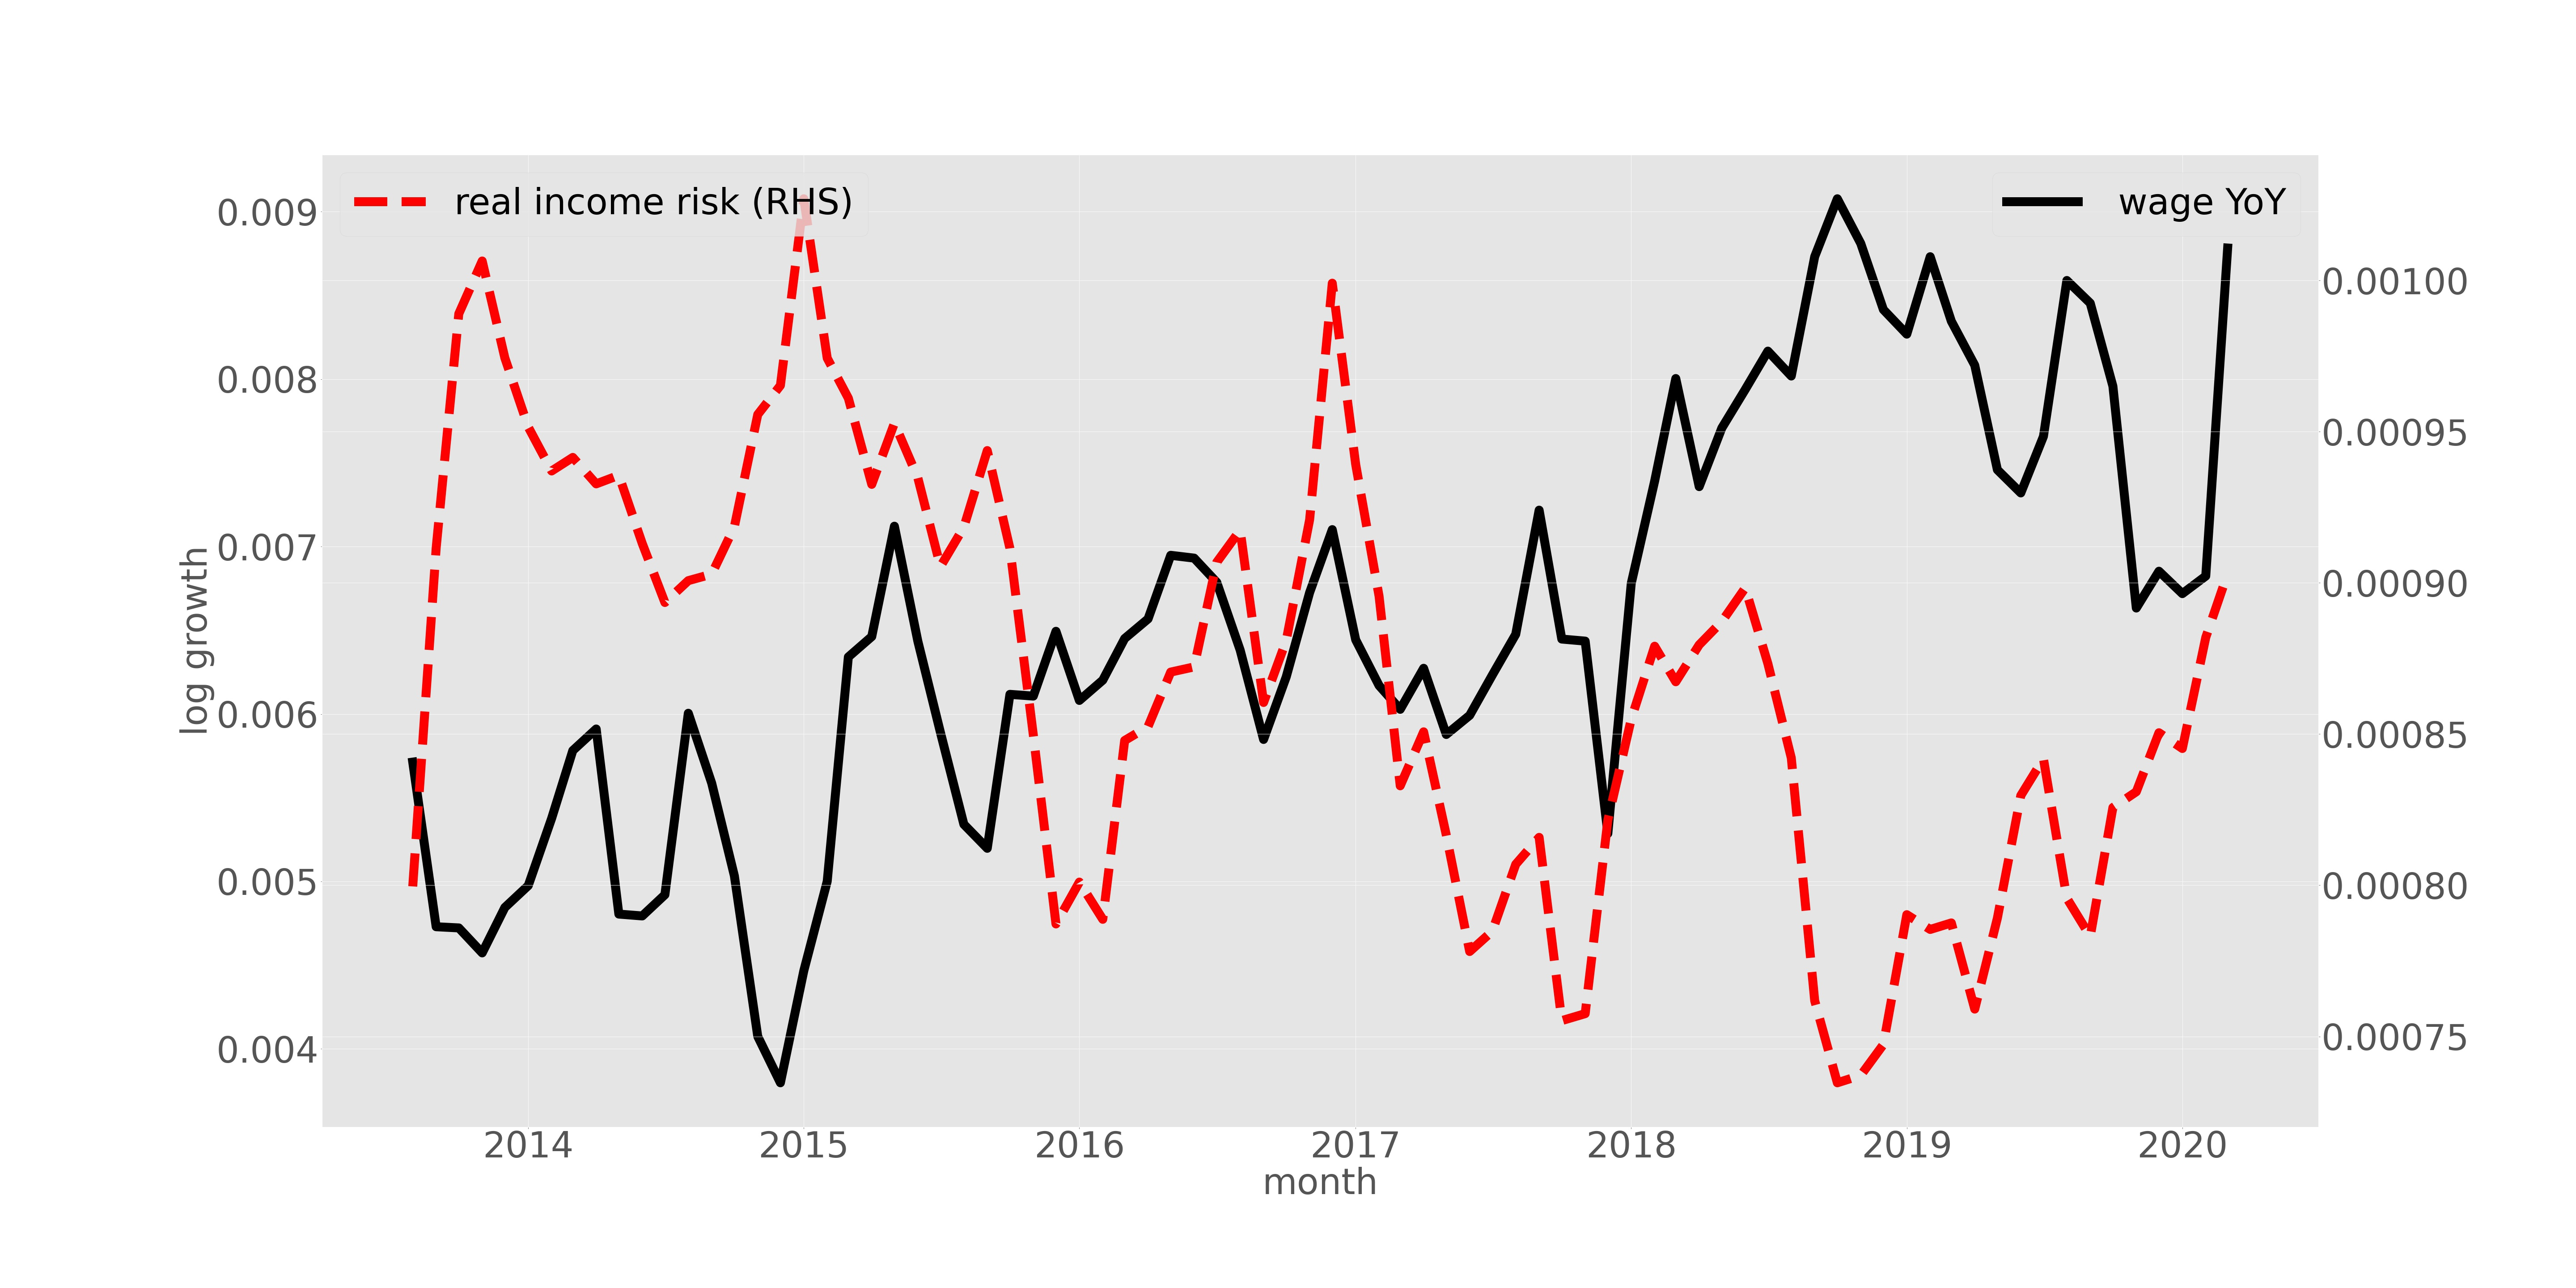
\includegraphics[width=\textwidth]{figures/tsMean3mvrvar_he.jpg}
	\end{figure}
	\quad  \hyperlink{appendix:tsMean3mvrexp_he}{\beamerbutton{expected growth}} 
\end{frame}


%\begin{frame}{Perceived \textcolor{blue}{real} income risks and past wage growth}
%	\begin{itemize}
%	\item $\overline{\text{rvar}_{t}} $
%	\item  $log(\text{wage}_t) - log(\text{wage}_{t-3})$
%\end{itemize}
%	\begin{figure}
%		\centering 
%		\label{ts_skew}
%		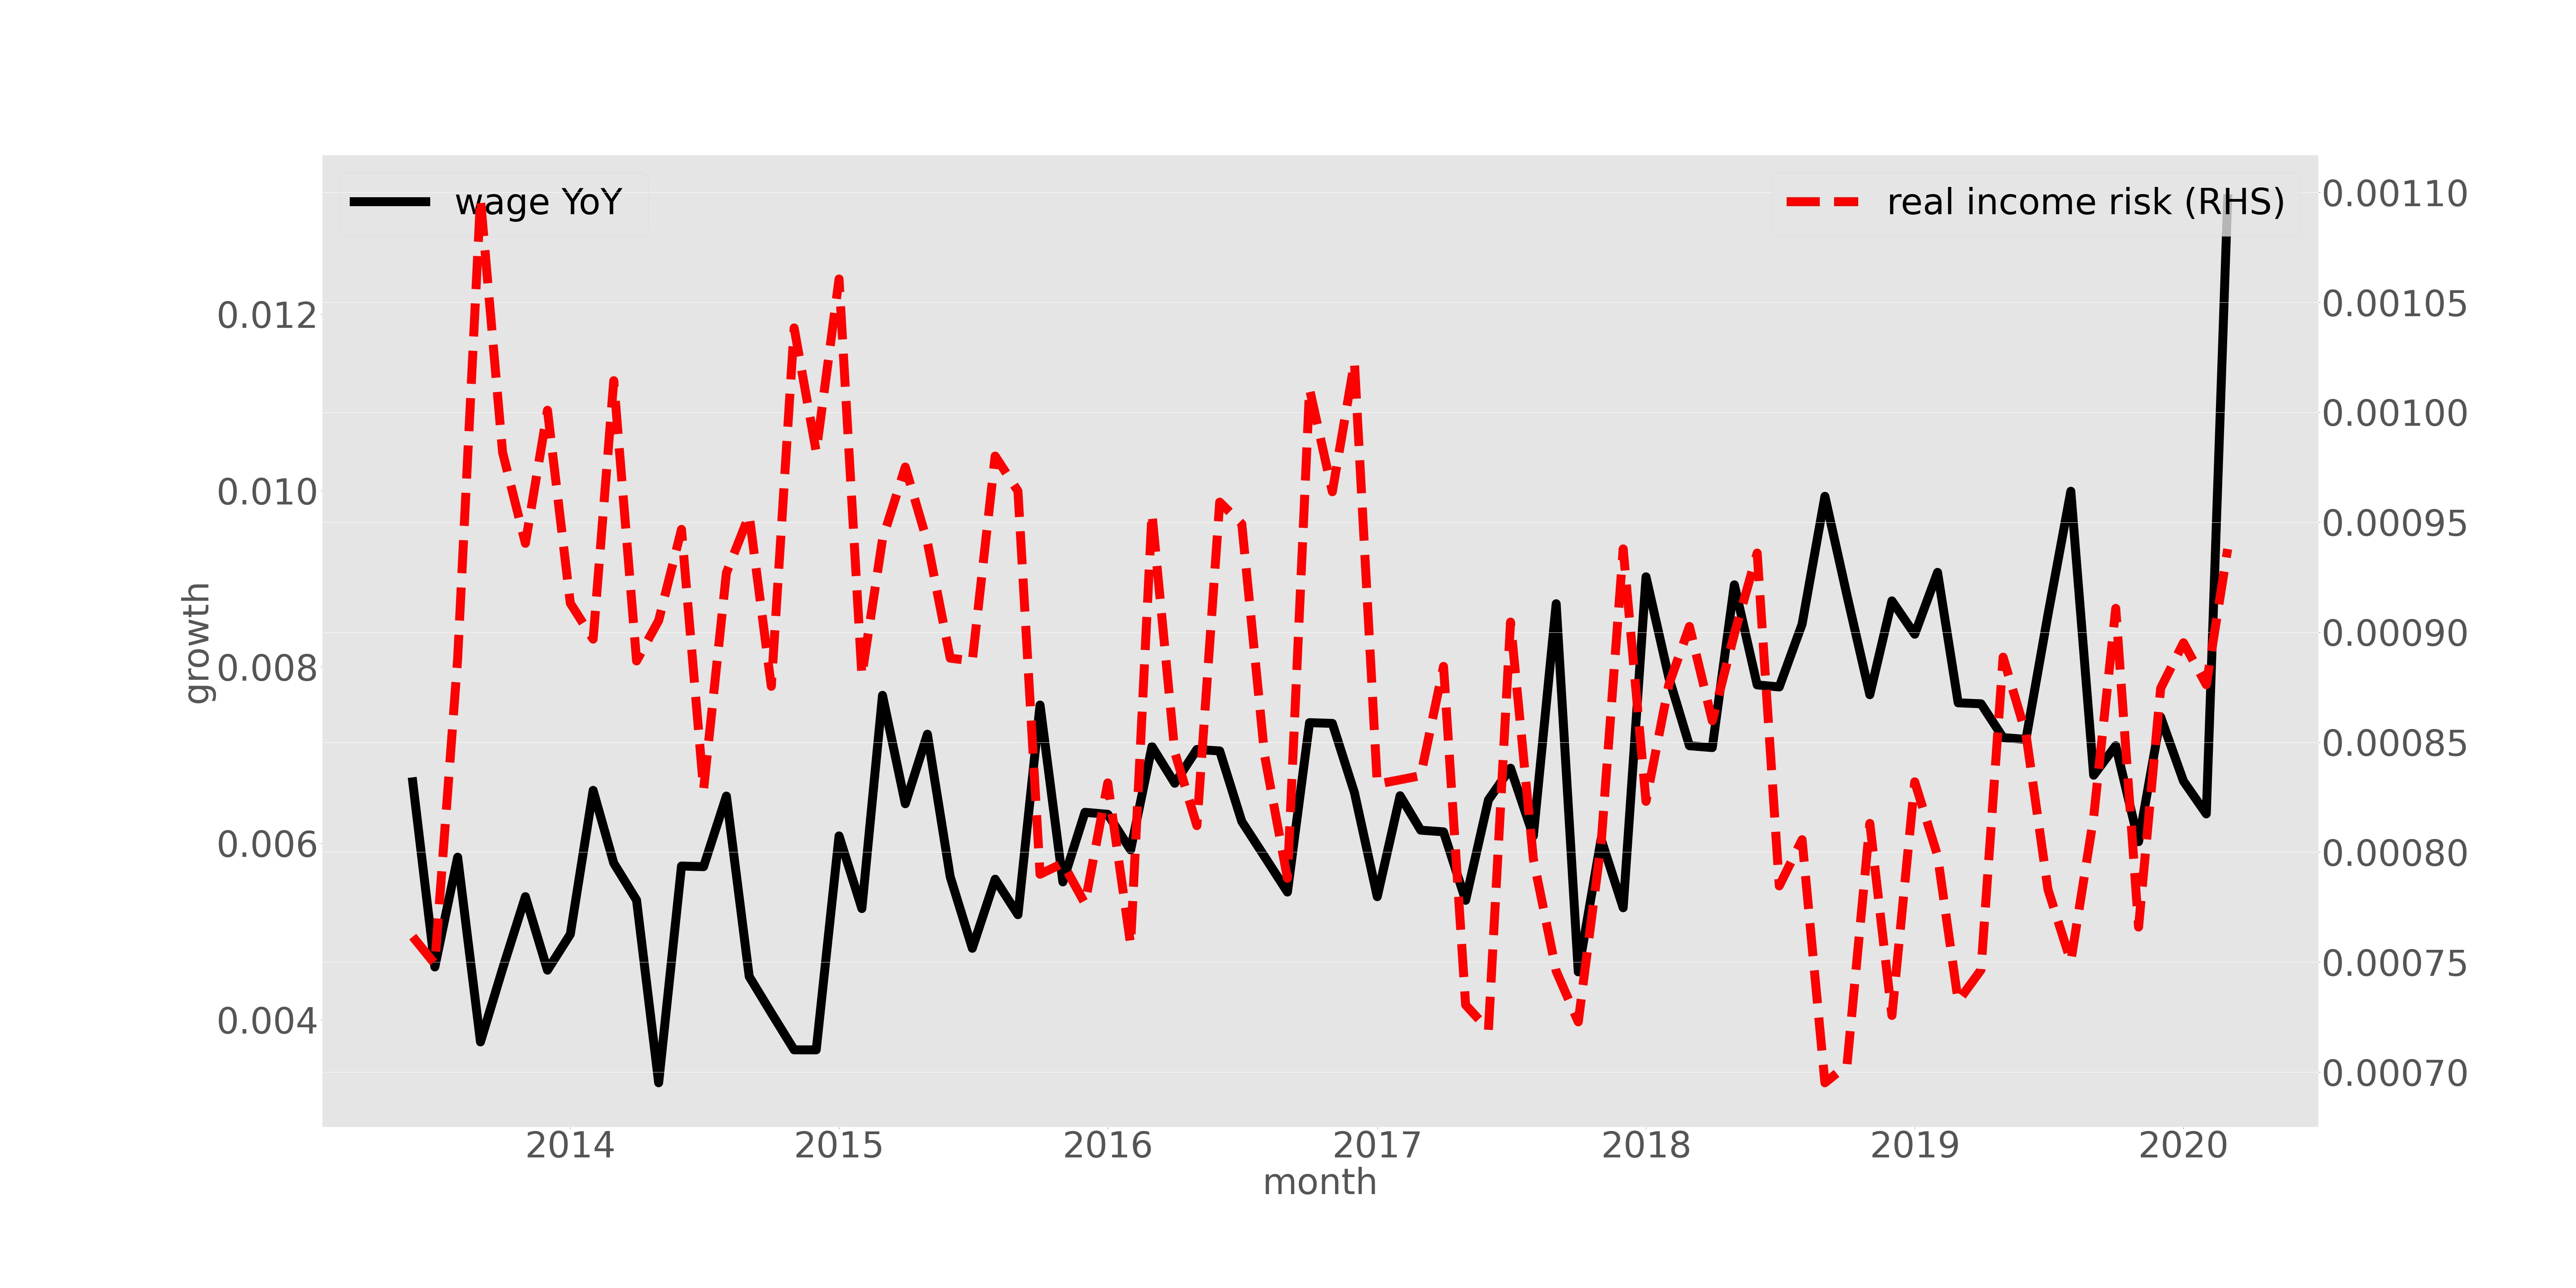
\includegraphics[width=\textwidth]{figures/tsMeanrvar_he.jpg}
%	\end{figure}
%\end{frame}



\begin{frame}{Perceived risks and current labor market condition}
	\begin{eqnarray*}
		\underbrace{\overline{\text{risk}_{t}}}_{\text{average perceived risk}} = \alpha + \textcolor{red}{\beta} \underbrace{(log(\text{wage}_{t-k/12}) - log(\text{wage}_{t-(k-3)/12}))}  _{\text{wage growth}}  + \epsilon_{i,t}	 \\
		\quad \forall k =0...4
	\end{eqnarray*}
	
	\begin{table}
		\centering
		%\caption{Correlation between Perceived Income Risks and Stock Market Return}
		\label{macro_corr_he}
		\adjustbox{max height=0.5\textheight, max width=\textwidth}{ 
		\begin{tabular}{lllll}
				\hline 
			& mean:var & mean:iqr & mean:rvar & mean:skew \\
				\hline 
			0 & -0.28**  & -0.42*** & -0.48***  & -0.02     \\
			1 & -0.42*** & -0.53*** & -0.51***  & 0.12      \\
			2 & -0.43*** & -0.48*** & -0.44***  & -0.01     \\
			3 & -0.43*** & -0.48*** & -0.42***  & -0.1      \\
			4 & -0.31*** & -0.41*** & -0.32***  & -0.21*   \\
			\hline 
		\end{tabular}
		}
	\end{table}
\begin{itemize}
	\item Counter-cyclical income risks: \cite{storesletten2004cyclical}, \cite{guvenen2014nature}, \cite{bayer2019precautionary}
	%\item Counter-cyclical skewness: \cite{guvenen_empirical_2009}, \cite{guvenen_inferring_2014} 
\end{itemize}
\end{frame}



\begin{frame}{Perceived risks and current labor market condition}
	\begin{eqnarray*}
		\underbrace{\overline{\text{risk}_{s,t}} }_{\text{median perceived risk in state $s$}}= r + \textcolor{red}{\psi} \underbrace{LM_{s,t}}_{\text{state labor market condition}}  + \eta_{s,t}
	\end{eqnarray*}
	\begin{table}
		\centering
		%\caption{Correlation between Perceived Income Risks and Stock Market Return}
		\label{macro_corr_he_state}
		\adjustbox{max height=0.5\textheight, max width=\textwidth}{ 
			\begin{tabular}{lllll}
				\hline 
				& (1)                & (2)                & (3)               & (4)               \\
				\hline 
				& log(var) & log(risk) & log(iqr) & log(iqr) \\
				\hline 
				wage growth & -0.05***           &                    & -0.03***          &                   \\
				
				& (0.01)             &                    & (0.01)            &                   \\
				unemp rate &                    & 0.04*              &                   & 0.04***           \\
				&                    & (0.02)             &                   & (0.01)            \\
				\hline 
				Observations      & 3529               & 3529               & 3546              & 3546              \\
				R-squared         & 0.023              & 0.020              & 0.025             & 0.028            \\
				\hline 
			\end{tabular}
		}
	\end{table}
\end{frame}

\subsection{Perceived unemployment risks}



\begin{frame}{Perceived unemployment risk and realized job separation rate}
	\begin{figure}
		\centering
		\label{ue_expectations}
		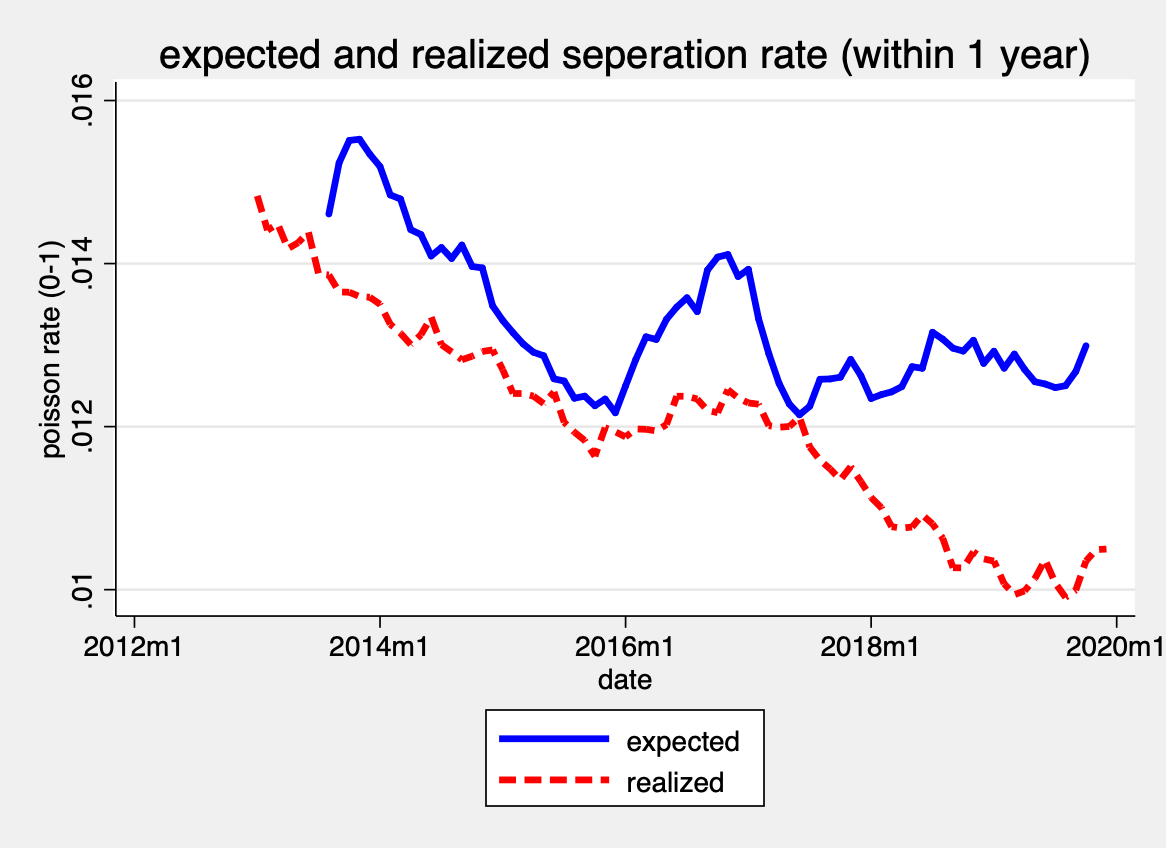
\includegraphics[width=0.7\textwidth]{figures/seperation_rate_1y}
	\end{figure}
	\begin{itemize}
	\item realized job separation rate is computed from CPS survey 
	\end{itemize}
\end{frame}




\subsection{Perceived risks and decisions}


\begin{frame}{Perceived risks and household spending}
	
	\begin{eqnarray*}
		E_{i,t} (\Delta c_{i,t+1}) = u_0 + \textcolor{red}{u_1} \overline{\text{risks}}_{i,t} (\Delta y_{i,t+1}) + \xi_{i,t}  
	\end{eqnarray*}
	\begin{table}
		\centering
		%\caption{Perceived income risks and household spending}
		\label{spending_reg}
		\adjustbox{max height=0.5\textheight, max width=\textwidth}{ 
			
\begin{tabular}{lllllll}
	\hline 
	& (1)      & (2)      & (3)      & (4)      & (5)      & (6)      \\
		\hline 
	perceived earning risk           & 8.394*** & 8.399*** & 3.642*** & 3.243*** &          &          \\
	& (1.175)  & (1.176)  & (0.533)  & (0.537)  &          &          \\
	&          &          &          &          &          &          \\
	perceived earning risk (nominal) &          &          &          &          & 3.656*** &          \\
	&          &          &          &          & (0.990)  &          \\
	&          &          &          &          &          &          \\
	perceived ue risk                &          &          &          &          &          & 0.353*** \\
	&          &          &          &          &          & (0.0553) \\
		\hline 
	R-squared                        & 0.0010 & 0.00282  & 0.928    & 0.928    & 0.941    & 0.633    \\
	Sample Size                      & 53178    & 53178    & 53178    & 53178    & 54584    & 6269     \\
	Time FE                          & No       & Yes      & No       & Yes      & Yes      & No       \\
	Individual FE                    & No       & No       & Yes      & Yes      & Yes      & Yes     \\
		\hline 
\end{tabular}
		}
	\end{table}
	\begin{itemize}
		\item  Higher perceived risks $\rightarrow$ higher expected spending growth. 
	\end{itemize}
\end{frame}

%\begin{frame}{\textcolor{red}{Counter-cyclical} perceived risks, continued}
%		\begin{figure}
%		\centering 
%		\label{var_experience_var}
%		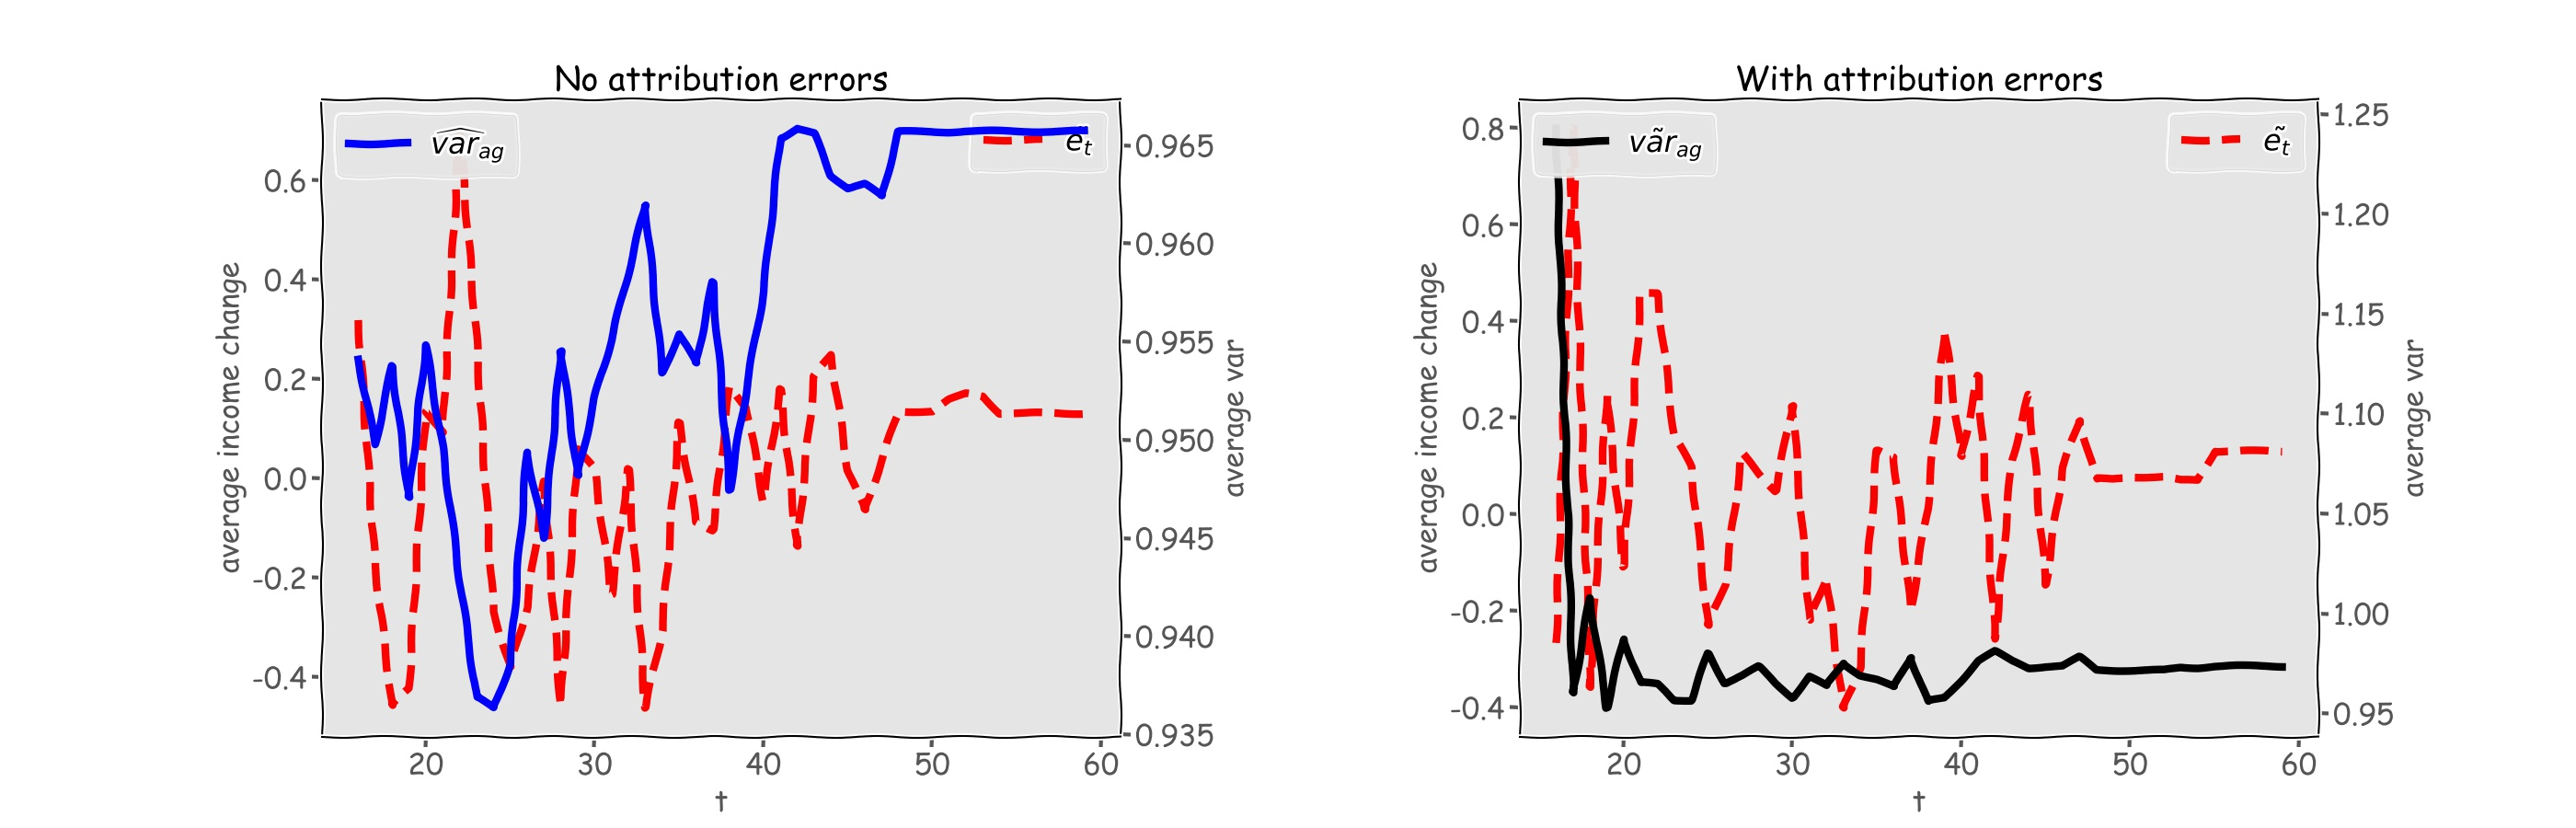
\includegraphics[width=\textwidth]{figures/var_recent_change_sim.jpg}
%	\end{figure}
%	\begin{figure}
%		\centering 
%		\label{var_experience_var}
%		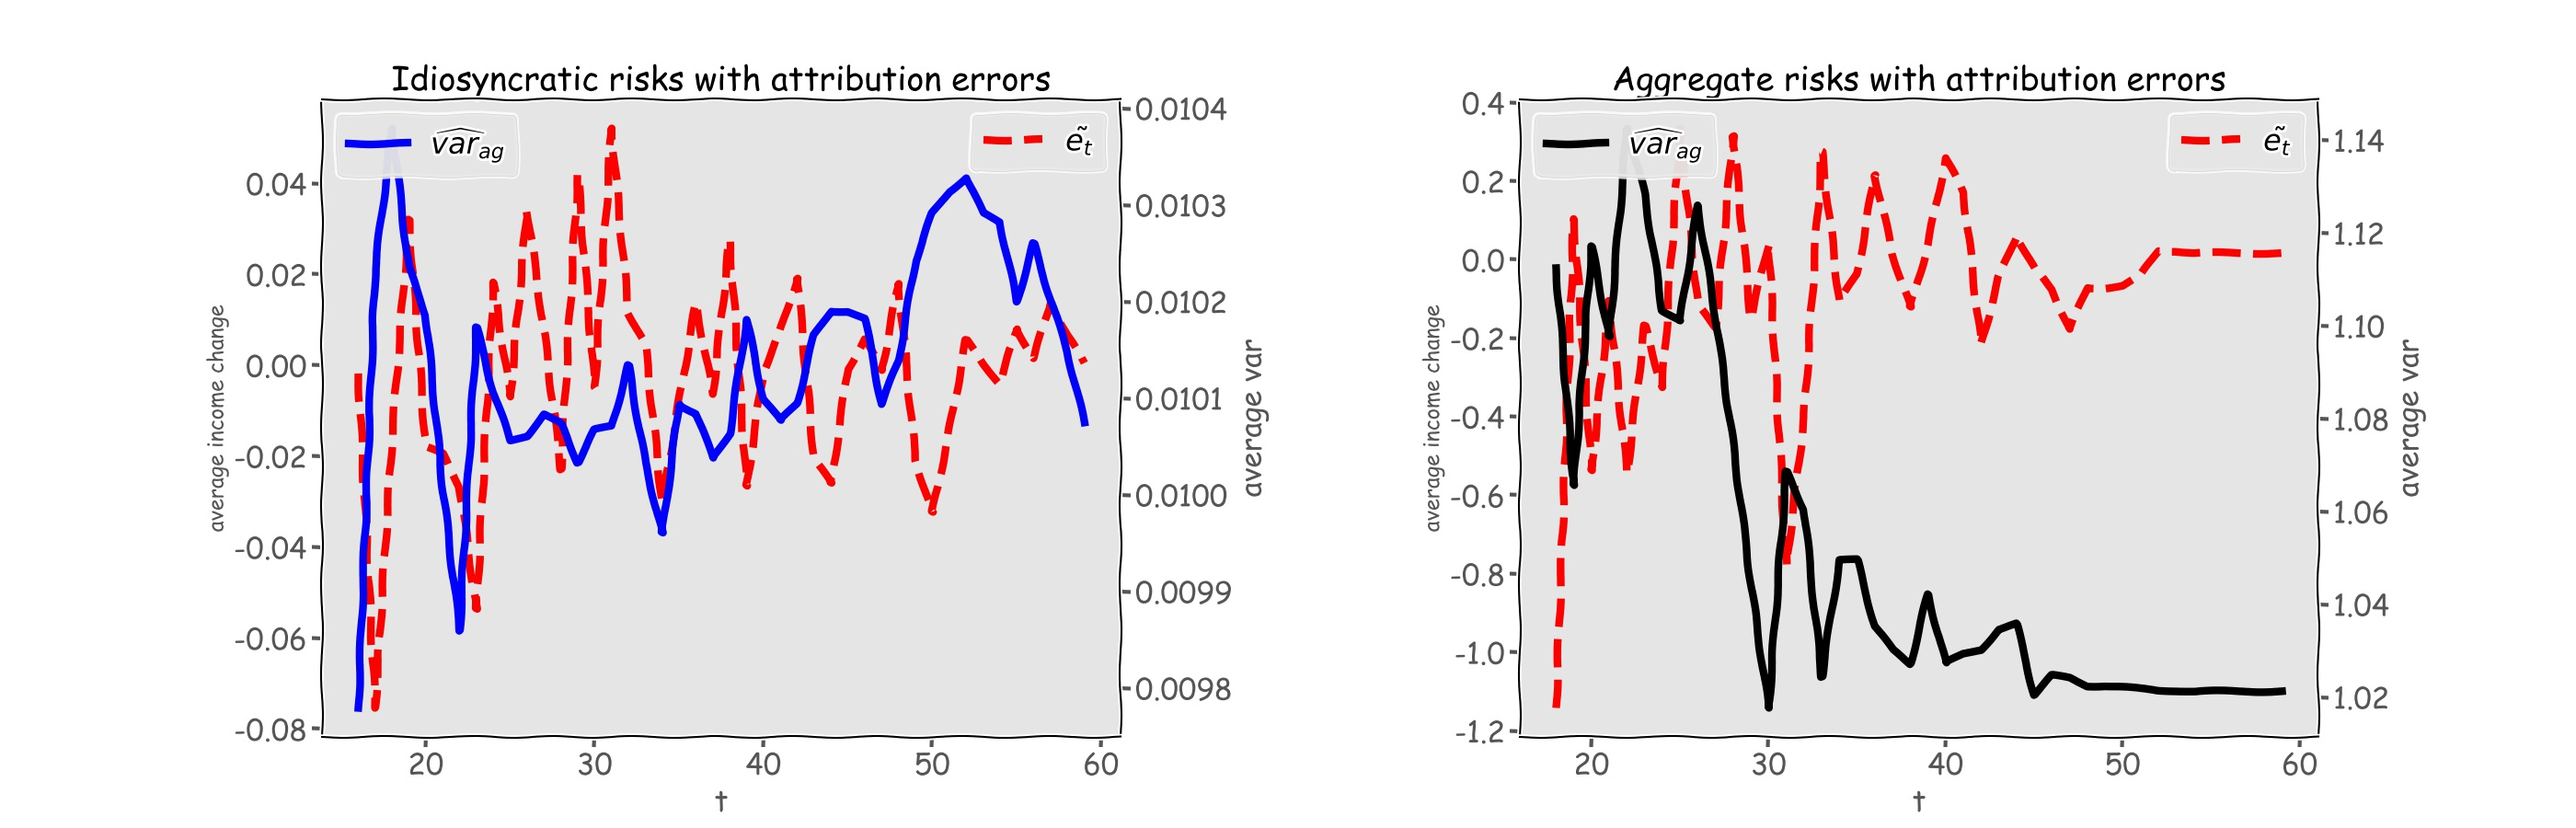
\includegraphics[width=\textwidth]{figures/var_recent_change_sim2.jpg}
%	\end{figure}
%\end{frame}


%\begin{frame}{Prediction 4. perceived risk declines over age}
%	\begin{figure}
%		\centering 
%		\label{var_experience_var}
%		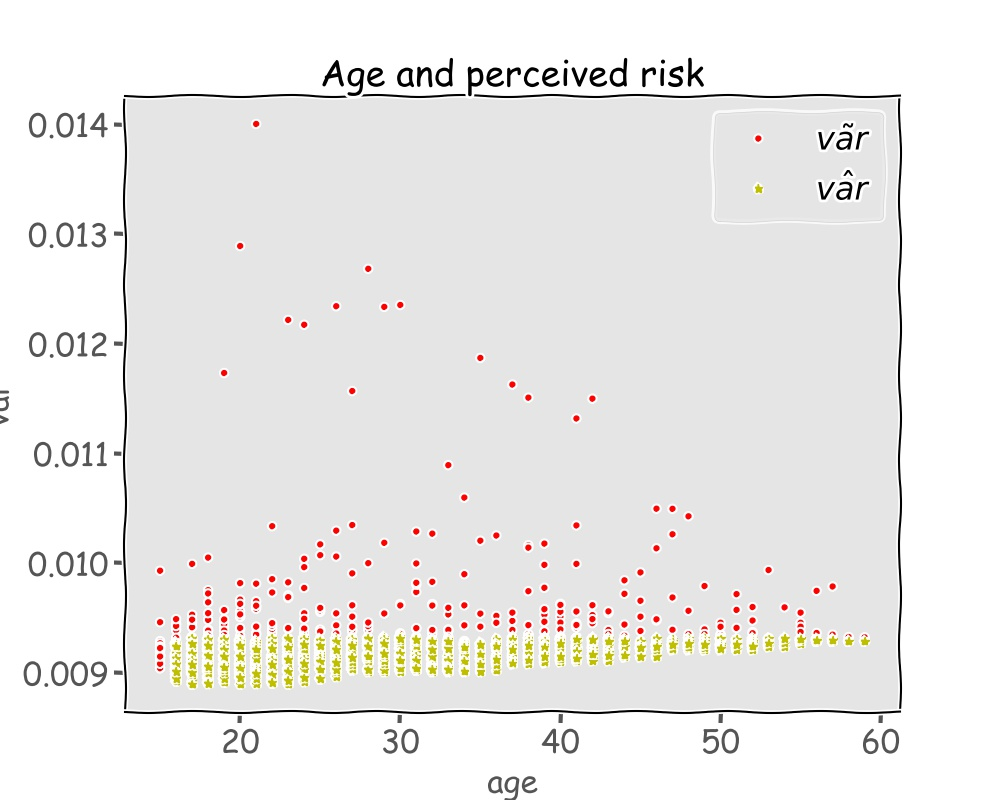
\includegraphics[width=0.7\textwidth]{figures/var_age_sim.jpg}
%	\end{figure}
%\end{frame}


%\begin{frame}{Prediction 3. skewed U-shaped income profile}
%	\begin{eqnarray}
%		\begin{split}
%			\tilde {Var}_{i,t}(\Delta y_{i,t+1})  = [(\sum^{t-c}_{k=0}\sum^{n}_{j=1}y^2_{j,t-k-1})^{-1}(1+\tilde\delta_{i,t}(n-1))y^2_{i,t} + 1] s^2_{i,t} 
%		\end{split}
%	\end{eqnarray}
%		\begin{figure}
%		\centering 
%		\label{var_experience_var}
%		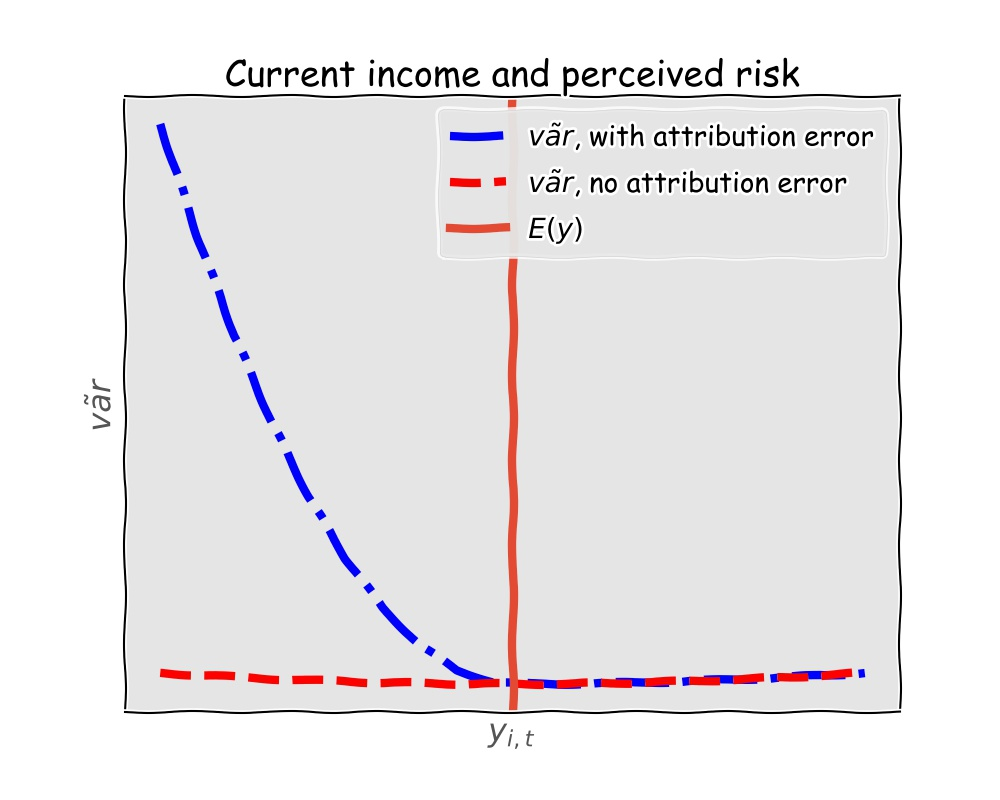
\includegraphics[width=0.6\textwidth, height = 0.6\textheight]{figures/var_recent.jpg}
%	\end{figure}
%\end{frame}



%\subsection{Simulation}	


%\begin{frame}{Simulated income profile}
%	\begin{figure}
%		\centering 
%		\label{var_experience_var}
%		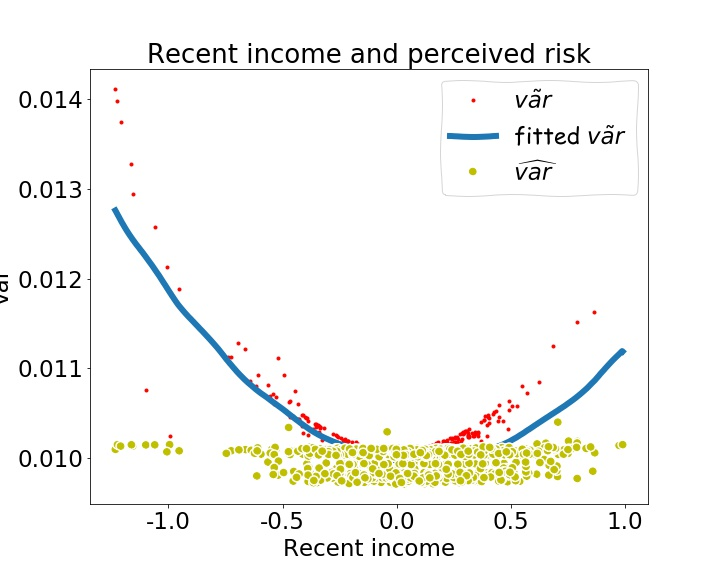
\includegraphics[width=0.7\textwidth]{figures/var_recent_sim.jpg}
%	\end{figure}
%\end{frame}



%\begin{frame}{Robustness}
%	\begin{itemize}
%		\item Permanent and transitory income risk 
%		\item Serial correlation 
%		\item Time-varying income risks 
%		\item More regressors 
%	\end{itemize}
%\end{frame}

\subsection{Summary of empirical findings}
\begin{frame}{Taking stock}
	
	\begin{itemize}
		\item People do have some clues 
		\begin{itemize}
			\item  consistent with inter-group differences in income volatility
			\item other covariates 
			\begin{itemize}
				\item $\downarrow$ with education, household income, being a male
				\item $\uparrow$  with numeracy score, self-employed job, perceived individual UE risks, aggregate UE expectations, experienced volatility 
			\end{itemize}
		\end{itemize}
		\pause
		\item But huge amount of heterogeneity remains
		\begin{itemize}
			\item including all above: $R^2 =0.10$
			\item individual fixed effects only: $R^2=0.71$
		\end{itemize}
		\pause
		\item Possible explanations
		\begin{itemize}
			\item ``superior information''/ unobserved heterogeneity
			\item state dependence: aggregate economy conditions matter  
			\item past dependence: experiences matters \cite{kuchler2019personal}
			\item intrinsic heterogeneity: some are more uncertain than the other \cite{ben2018expectations} 
		\end{itemize}
	\end{itemize} 
\end{frame}


\begin{comment}
	
\begin{frame}{A simple model of risk perception}
	\label{model}
	\begin{itemize}
		\item Under FIRE 
		\begin{equation*}
			\begin{split}
				&{ Var}^*_{i,c,t}(\Delta y_{i,c,t}) =  \sigma^2_{\psi,c} + \sigma^2_{\epsilon,c} 
			\end{split}
		\end{equation*}
		\item  Under imperfect understanding
		\begin{itemize}
			\item $\phi$ and $\sigma^2_{\epsilon,c}$ are not perfectly known 
			\item all realized shocks are perfectly observed  
		\end{itemize}
	\end{itemize}
	\begin{equation*}
		\begin{split}
			& \widetilde{ Var}_{i,c,t}(\Delta y_{i,c,t+1}) =  \sigma^2_{\psi,c} + \tilde \sigma^2_{\epsilon,c,t} \\
			&\textcolor{blue}{\text{Experience-dependence: }}	\tilde \sigma^2_{\epsilon,c,t} =  \frac{\overbrace{Var_{i,c,t}(\eta_{i,c,t})}^{\text{experienced volatility}} }{1+\tilde \phi^2_{i,c,t}} \\
			&\textcolor{blue}{\text{State-dependence: }}		\tilde \phi_{i,c,t} =  \delta(\epsilon_{i,c,t})  
		\end{split}
	\end{equation*}
\end{frame}

\end{comment}

\begin{frame}{Implications for consumption/saving}
	\begin{itemize}
		\item On \textcolor{red}{level} of aggregate savings
	\begin{enumerate}
		\item $\downarrow$ \textcolor{blue}{lower PR}: lower precautionary saving motives $\rightarrow$ less liquid holding $\rightarrow$ higher MPC
		\pause
		\item $\uparrow$  \textcolor{blue}{state-dependence}: a mean-preserving spread in risks
	 $\rightarrow$  more precautionary savings \cite{caballero1990consumption}
	 	\pause
	\item $\uparrow$ \textcolor{blue}{extrapolation}: lower income/unemployment $\rightarrow$ higher PR $\rightarrow$ intensified precautionary motive 
		\pause
		\item $\uparrow$ \textcolor{blue}{counter-cyclical risks}:  amplified business cycle fluctuations \cite{bayer2019precautionary}
	\end{enumerate}
\pause 
\item On \textcolor{red}{wealth inequality}
\begin{itemize}
	\item 	$\uparrow$ Direct effect: \textcolor{blue}{heterogeneous PR} $\rightarrow$ heterogeneity in saving/wealth
\item $\uparrow$ Indirect effect: \textcolor{blue}{lower PR} $\rightarrow$ lower self-insurance $\rightarrow$ higher  ex-post wealth inequality
	\end{itemize}
	\end{itemize}
\end{frame}


\section{Model}

\begin{frame}{Model overview}
	\begin{itemize}
		\item Overlapping generation 
		\item General equilibrium 

		\item Uninsured idiosyncratic income risks
		\begin{itemize}
		\item Permanent+ transitory productivity shock
		\item Persistent unemployment spells
		\end{itemize}
	\item No aggregate risk a la \cite{krusell1998income} 
		\item A blend of \cite{huggett1996wealth} and \cite{carroll1997buffer}
		\item Single one risk-free asset
	\item Allowing for \textcolor{red}{subjective} risk perceptions 
	\begin{itemize}
		\item Individuals swing between low/high risk perceptions
	\end{itemize}

	\end{itemize}
\end{frame}

\begin{frame}{Benchmark model (objective risk perceptions)}

\begin{equation*}
	\textrm{max}\quad  \mathbb{E}\left[\sum^{\tau=L-1}_{\tau=0}(1-D)^\tau\beta^\tau u(c_{i,\tau})\right] 
\end{equation*}



\begin{equation*}
	\begin{split}
		& \underbrace{a_{i,\tau}}_{\text{Savings}} = \underbrace{m_{i,\tau}}_{\text{Cash in hand}} - c_{i,\tau} \\
		& b_{i,\tau+1} = a_{i,\tau} R  \\
		& m_{i,\tau+1}   = b_{i,\tau+1}+(1-\underbrace{\lambda}_{\text{Income tax}})y_{i,\tau+1}\\
		& a_{i,\tau} \geq 0 
	\end{split}
\end{equation*}


\begin{itemize}
	\item CRRA: $u(c) = \frac{c^{1-\rho}}{1-\rho}$
	\item Work age: $\tau=1, 2...,T$ (since entering job market) 
	\item Life length: $\tau=1, 2...,L$  (since entering job market)
	\item Survival probability: 1-D
\end{itemize}

\end{frame}



\begin{frame}{Income process}
	\begin{itemize}
		\item income
	\begin{equation*}
		\begin{split}
			y_{i,\tau} = n_{i,\tau}W  \\
			n_{i,\tau} = p_{i,\tau}\xi_{i,\tau}
		\end{split}
	\end{equation*}
	\item permanent component 
\begin{equation*}
	\begin{split}
		p_{i,\tau} = G_\tau p_{i,\tau-1}\psi_{i,\tau}, \quad
		log (\psi_{i,\tau}) \sim N(-\sigma^2_{\psi}/2,\textcolor{red}{\sigma^2_{\psi}})
	\end{split}
\end{equation*}
	\item persistent/transitory component 
\begin{equation*}
	\begin{split}
\xi_{i,\tau} =   \left\{
\begin{array}{ll}
	\theta_{i,\tau} \quad \text{if} \quad \nu_{i,\tau} =0 \quad \& \quad  \tau \leq T, \quad log(\theta_{i,\tau}) \sim N(-\frac{\sigma^2_\theta}{2},\sigma^2_\theta)\\
	\zeta \quad \text{if} \quad \nu_{i,\tau} = 1 \quad \& \quad \tau \leq T  \\
	\mathbb{S} \quad \text{if}  \quad \tau > T
\end{array} \right. 
\end{split}
\end{equation*}
	\item transition probability between $\nu=1$ and $\nu=0$
\begin{equation*}
	\pi_{i,\tau+1|\tau} = 
	\begin{bmatrix} 
		\textcolor{red}{\mho} & 1-\mho  \\
		1-E & \textcolor{red}{E}
	\end{bmatrix}
	\quad
\end{equation*}
	\end{itemize}
\end{frame}


\begin{frame}{Objective  versus subjective profile}
	\begin{itemize}
		\item \textcolor{blue}{objective}: agents perceive $\underbrace{\Gamma =\{\sigma^2_\psi,\sigma^2_\theta,\mho,E\}}_{\text{income risk parameters}}$ 
			\item \textcolor{blue}{subjective with state-dependence}: each agent $i$ swings between two  subjective risk state  $\tilde \Gamma_{i,\tau} = \tilde \Gamma_l$ and $\tilde \Gamma_{i,\tau} = \tilde \Gamma_h$, with transition matrix $\Omega$. 
			\begin{itemize}
				\item heterogeneity in risk perceptions 
			\end{itemize}
			\item \textcolor{blue}{subjective model with extrapolation}:  $\tilde \Gamma_{i,\tau}$ depends on employment status $\nu_{i,\tau}$, i.e. $\tilde \Gamma_{i,\tau}(\nu_{i,\tau}=0) = \tilde \Gamma_l$ and $\tilde \Gamma_{i,\tau}(\nu_{i,\tau}=1) = \tilde \Gamma_h$
	\end{itemize}
\end{frame}


\begin{frame}{Why \textcolor{red}{subjective} risk perceptions?}
	\begin{itemize}
		\item I don't take a stance on if agents perceptions are correct or wrong
		\item It could be due to unobserved information to economists, or because of psychological reasons
		\item The subjective risk profile is disciplined by the survey data 
		\item Risk parameters are exogenous to the model, therefore, does not contradict with rational expectation. 
	\end{itemize}
\end{frame}

\begin{frame}{Economic environment}
	\begin{itemize}
		\item \textcolor{blue}{Technology}
		\begin{equation*}
			Y = Z K^{\alpha}N^{1-\alpha}
		\end{equation*}
	\pause
		\item \textcolor{blue}{Government (balance budget)}
		\begin{equation*}
			\label{Eq:gov}
			\lambda \left[ 1-\text{fraction of unemp}  + \zeta \text{fraction of unemp}\right]  = \zeta \text{fraction of unemp}   
		\end{equation*}
	\pause
		\item \textcolor{blue}{Demographics}
		\begin{itemize}
			\item Stable age distribution  $\{\mu_\tau \}_{\mu=1,2,..L}$ 
			\begin{equation*}
				\begin{split}
			& \mu_{\tau+1} = (1-D)\mu_{\tau} \\ &\sum^{L}_{\tau=1}\mu_{\tau} = 1
			\end{split}
			\end{equation*}
		\end{itemize}
	\pause
		\item \textcolor{blue}{Accidental bequests}
		 \begin{itemize}
		 	\item Newborn starts with a bank-balance equal to $0-1$ fraction of the lump-sum of the accidental deceased's wealth 
		 \end{itemize}
	\end{itemize}
\end{frame}


\begin{frame}{Value functions under different profiles}
	\begin{itemize}
		\item \textcolor{blue}{objective}: 
		
		\begin{equation*}
			\begin{split}
				V_{\tau}(\underbrace{\nu_{i,\tau}, m_{i,\tau}, p_{i,\tau}}_{x_{i,\tau}})  =  & \underset{\{c_{i,\tau},a_{i,\tau}\}}{\textrm{max}} \quad   u(c_{i,\tau}) \\
		& +  (1-D)\beta \mathbb{E}_{\tau}\left[V_{\tau+1}((\nu_{i,\tau},m_{i,\tau+1}, p_{i,\tau+1})\right] 
			\end{split}
		\end{equation*}
		\item \textcolor{blue}{subjective}: 
		
		\begin{equation*}
			\begin{split}
				\tilde V_{\tau}(\underbrace{\textcolor{red}{\tilde \Gamma_\tau}, \nu_\tau, m_\tau, p_\tau}_{\tilde x_{i,\tau}}) = & \underset{\{c_\tau\}}{\textrm{max}} \quad  u(c_\tau) \\
				&  + (1-D)\beta \mathbb{E}_{\tau}\left[\tilde V_{\tau+1}(\textcolor{red}{\tilde \Gamma_{\tau+1}}, \nu_\tau,m_{\tau+1}, p_{\tau+1})\right] 
			\end{split}
		\end{equation*}
	\end{itemize}
\end{frame}


\begin{frame}{Evolution of the distribution over state variables}
		\begin{itemize}
		\item \textcolor{blue}{objective}: 
		
		\begin{equation*}
			\label{Eq:DistDyn}
			\psi_{\tau}(B)=\int_{x \in X} \underbrace{P(x, \tau-1, B) \mathrm{d}}_{\text{transition funcs}} \psi_{\tau-1} \quad \text { for all } \quad B\in B(X)
		\end{equation*}
	
	\begin{itemize}
		\item $B(X)$:  distribution measure on state space $X$
		\item $\psi_{\tau}$: distribution over state variables $x$ for agents in age $\tau$
		\item $\psi_{1}$ depends on initial draws of income shocks 
	\end{itemize}

		\item \textcolor{blue}{subjective}: 
		
		\begin{equation*}
			\label{Eq:DistDynSub}
			\tilde \psi_{\tau}(\tilde B)=\int_{\tilde x \in \tilde X} \tilde P(\tilde x, \tau-1, \tilde B) \mathrm{d} \tilde \psi_{\tau-1} \quad \text { for all } \quad \tilde B \in \tilde B(X)
		\end{equation*}
	
	\end{itemize}
\end{frame}

\begin{frame}{Stationary equilibrium (StE)}
\begin{itemize}
	\item Optimal consumption and saving policies given $W$, $R$, $\lambda$
	\item Distribution evolution consistent with optimal $c$ and $a$ policies and exogenous probabilities of income/beliefs
	\item The factor markets are clearing. 
	\begin{equation*}
		\begin{split}
			\sum_{\tau} \mu_{\tau} \int_{X}a(x, \tau) \mathrm{d} \psi_{\tau}=K \\
			\sum^{T-1}_{\tau=0} \mu_{\tau} \int_{X}  \mathbbm{1}(\nu_{i,\tau} =1)n(x, \tau) \mathrm{d} \psi_{\tau}=N
		\end{split}
	\end{equation*}
\item Firm optimization under competitive factor markets.
$$W = Z(1-\alpha) (K/N)^\alpha $$
$$R = 1+Z\alpha (K/N)^{\alpha-1} - \delta$$
\item Newborn's bank balance equal to accidental bequests
\item Balanced government budget 
\end{itemize}
\end{frame}

\begin{comment}
	
\begin{frame}{Qualitative model implications}
	\begin{itemize}
		\item Heterogeneity in PR
		\begin{itemize}
			\item Direct effect: heterogeneity in precautionary wealth /$MPC$
		\end{itemize}
		\item Lower PR
		\begin{itemize}
			\item Lower wealth holdings of all groups 
			\item Indirect effect: lower ex-ante precautionary motives $\rightarrow$ ex-post lower degree of self-insurance $\rightarrow$ more wealth inequality 
		\end{itemize}
	\end{itemize}
\end{frame}
\end{comment}

\begin{frame}{Estimation of subjective 
risk profile}
\label{RegimeEstimation}

\begin{equation*}
	\begin{split}
&	\underbrace{\tilde \Gamma^s_{i,t}}_{\text{reported PR}} = \underbrace{\tilde \Gamma_l + \mathbbm{1}(\overbrace{J_{i,t}}^{\text{Hidden state}}= 1)( \tilde \Gamma_h -\tilde \Gamma_l)}_{\tilde \Gamma_{i,t}} +\xi_{t}+\eta_{i}+ \epsilon_{i,t}\\
& \text{Prob}(J_{i,t+1}|J_{i,t}) = \Omega
\end{split}
\end{equation*}

%\begin{equation*}
%	\begin{split}
%		\log(\tilde {\text{var}}_{i,t})= (12+\frac{1}{12\kappa^2})\tilde \sigma^2_{i,t,\psi} + \xi_{t}+\eta_{i}+ \epsilon_{i,t}
%	\end{split}
%\end{equation*}
\begin{itemize}
	
	\item $J_{i,t} =0$ for low and $=1$ for high PR state
	\item a short time series of $\tilde \Gamma_ {i,t}$ for many $i$s observed in the survey 
	\item $\{\tilde \Gamma_l\,\tilde \Gamma_h,\Omega\}$ can be estimated by $MLE$
	%\item $\kappa$: externally assumed ratio of permanent and transitory risks $\frac{\tilde \sigma_{i,t,\psi}}{\tilde \sigma_{i,t,\theta}}$
	\item a modified \cite{hamilton1989new} 2-regime-switching model 
	\item $J_{i.t}$ can be also dependent upon business cycles 
\end{itemize}
\hyperlink{appendix:RegimeEstimationDetail}{\beamerbutton{More details}} 
\end{frame}



\begin{comment}

\begin{frame}{Illustration: lower (expected) risk $\rightarrow $  higher consumption}
	\begin{figure}[!ht]
		\caption{Consumption functions under objective and subjective risk profiles}
		\label{fig:comparison1}
		\begin{center}
			\adjustimage{max size={0.8\linewidth}{0.5\paperheight}}{figures/comparison1.png}
		\end{center}
	\end{figure}

\begin{itemize}
	\item C depends on the individual's subjective risk perceptions, expected income risks  at the state $\tilde \Gamma$ 
\end{itemize}

\end{frame}

\begin{frame}{Illustration: intensified precautionary saving motive}

\begin{figure}[!ht]
	%\caption{Consumption functions under objective and state-dependent risk profiles}
	\label{fig:comparison2}
	\begin{center}
		\adjustimage{max size={0.8\linewidth}{0.5\paperheight}}{figures/comparison2.png}
	\end{center}
\end{figure}


\end{frame}

\end{comment}


\begin{frame}{Extensions: additional heterogeneity in $MPC$}

\begin{itemize}
	\item Heterogeneous time preferences
\begin{itemize}
	\item Ex-ante differences in $\beta$, a la \cite{krusell1998income,carroll2017distribution,krueger2016macroeconomics}.
\end{itemize}
	\item Costly adjustments
	\begin{equation*}
		\begin{split}
			& V_{i,\tau}(c_{i,\tau-1},x_{i,\tau}) = \textrm{max} \quad \{V^A_{\tau}(x_{i,\tau})-\chi,V^N_{\tau}(c_{i,\tau-1},x_{i,\tau})\} \\
			& V^A_{\tau}(x_{i,\tau}) = \underset{\{c_{i,\tau}\}}{\textrm{max}} \quad u(c_{i,\tau}) + (1-D)\beta \mathbb{E}_{\tau}\left[V_{\tau+1}(x_{i,\tau+1})\right]  \\
			& V^N_{\tau}(c_{i,\tau-1},x_{i,\tau}) =  u(c_{i,\tau-1}) + (1-D)\beta \mathbb{E}_{\tau}\left[V_{\tau+1}(c_{i,\tau},x_{i,\tau+1})\right]
		\end{split}
	\end{equation*}
	\begin{itemize}
		\item Utility cost from adjusting consumption in each period
		\item To introduce extensive margin of consumption change and match high $MPC$ from data 
	\end{itemize}
\end{itemize}
 \end{frame}




\section{Conclusion}


\begin{frame}{Summary}
	
	\begin{itemize}
 	\item Survey data can inform incomplete-market macro models 
 	\begin{itemize}
 		\item Direct evidence for heterogeneity in perceptions that matter
 		\item Closer to agents' information set that truly affects their decisions
 	\end{itemize}
	\item No need to make stringent assumptions on expectation formation
	\item More work needed on understanding risk perception formation  
	\end{itemize}
\end{frame}



%%%%%%%%%%%%%%%%%%%%%%%%%%

%% sumplement 

\section*{Appendix}



\begin{frame}{Within-group dispersion in nominal PR}
	\label{appendix:incstd}
	\begin{figure}
		\centering
		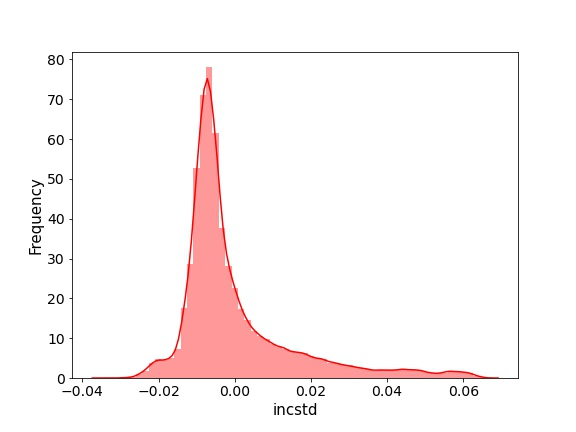
\includegraphics[width=0.65\textwidth]{figures/hist_incstd.jpg}
	\end{figure}
	\begin{itemize}
		\item  residuals controlling for observables /time fixed effects
		\item average PR:  $2.1\%$ in std; 10/90 IQR: $3.2\%$ in std \quad \hyperlink{rincstd_hist}{\beamerbutton{Back}}    
		% \item just a lower bound: before adjustment of unemployment risk 
	\end{itemize}
\end{frame}


\begin{frame}{Within-group dispersion in PR skewness}
	\label{appendix:incskew}
	\begin{figure}
		\centering
		%			\begin{subfigure}[b]{0.45\textwidth}
		%			\centering
		%			\caption{income risks (nominal)}
		%		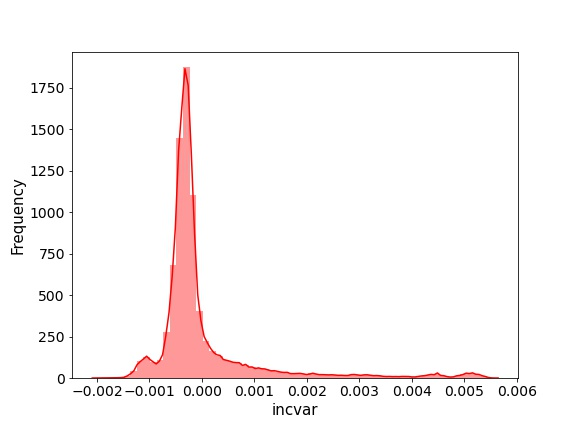
\includegraphics[width=\textwidth]{figures/hist_incvar.jpg}
		%		\end{subfigure}
		%	\begin{subfigure}[b]{0.45\textwidth}
		%		\centering
		%		\caption{income risks}
		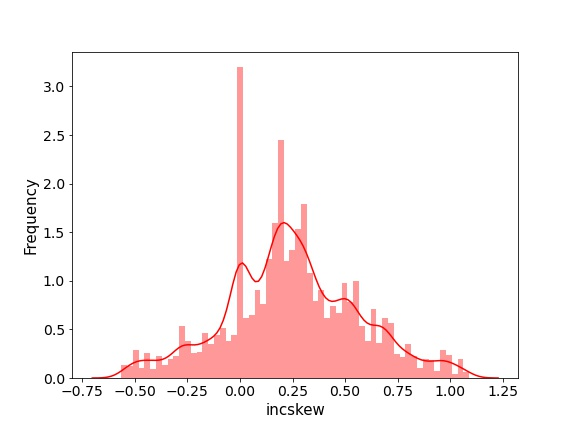
\includegraphics[width=0.65\textwidth]{figures/hist_incskew.jpg}
		%	\end{subfigure}
	\end{figure}
	\begin{itemize}
		\item  residuals controlling for observables / time fixed effects
		%\item average PR:  $3.5\%$ in std; 10/90 IQR: $6.4\%$ in std 
			\quad \hyperlink{rincstd_hist}{\beamerbutton{Back}}    
		% \item just a lower bound: before adjustment of unemployment risk 
	\end{itemize}
\end{frame}


\begin{frame}{Appendix: PR by age}
	\begin{figure}[ht]
		%\caption{Perceived Risk} 
		\label{appendix:age_compare_figure}
		\centering
		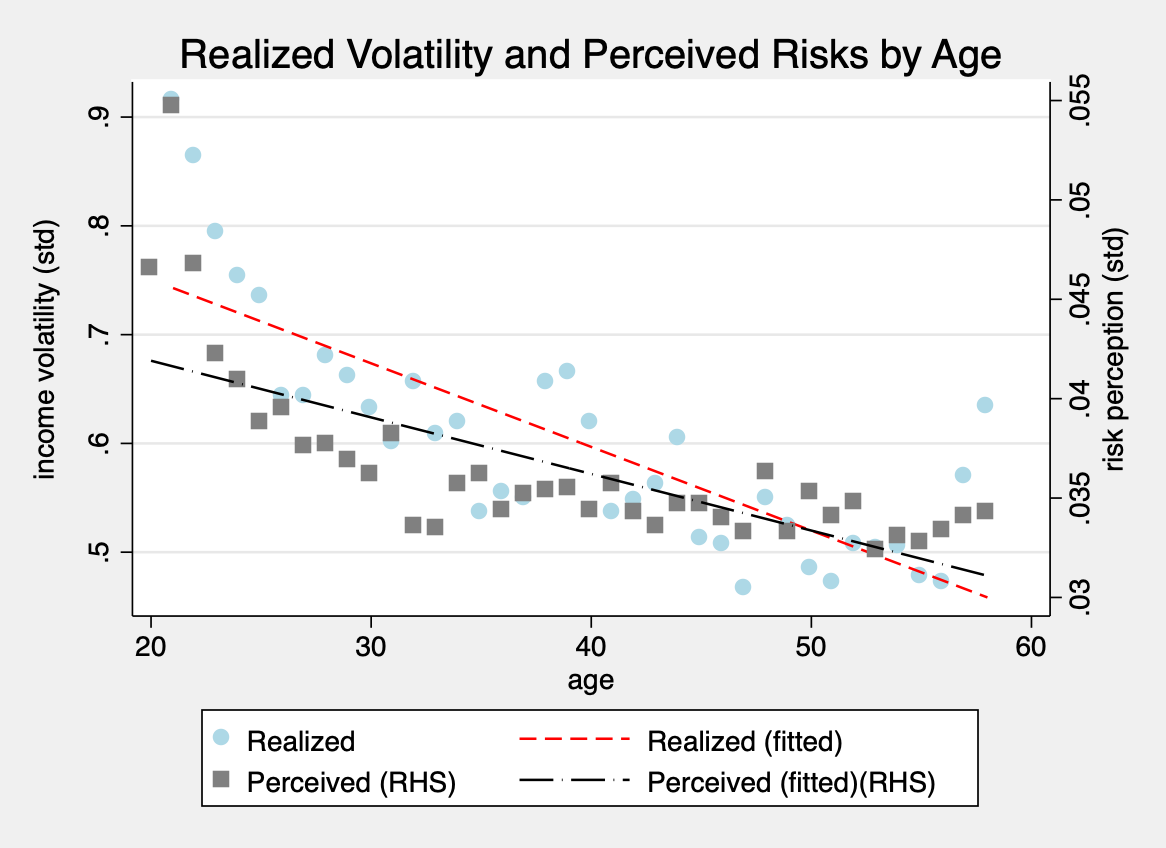
\includegraphics[width=0.7\textwidth]{figures/real_log_wage_shk_gr_by_age_compare.png}
	\end{figure}
	\begin{itemize}
		\item e.g. a 35-year old   \quad  \hyperlink{age_compare}{\beamerbutton{Back}} 
		%	\item in line with existing findings, for instance  
		%	\cite{bloom2018great}. 
	\end{itemize}
\end{frame}


\begin{frame}{Permanent versus transitory risks } 
	\label{appendix:monthly_decomposition_compare_psid}
	\begin{figure}[ht]
		%\caption{Perceived Risk} 
		\centering
		\begin{subfigure}[b]{0.44\textwidth}
			\caption{permanent}
			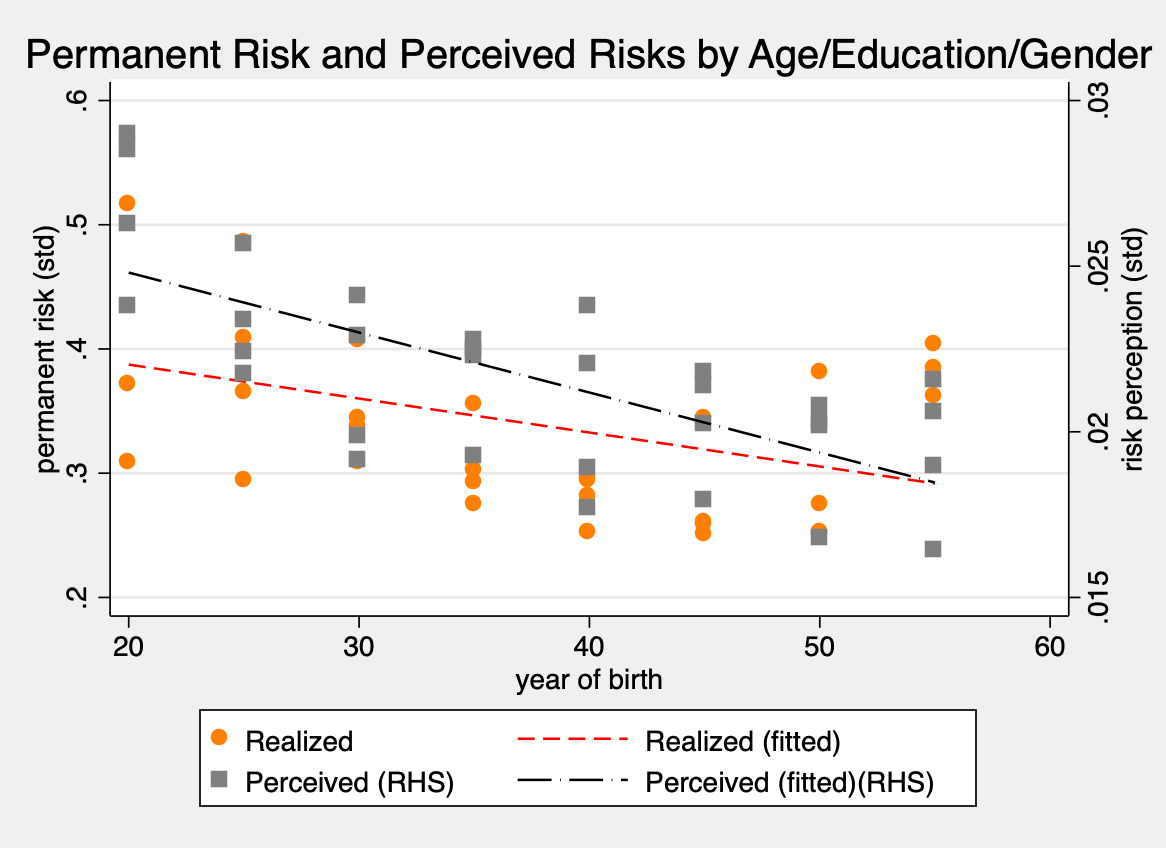
\includegraphics[width=\textwidth]{figures/log_wage_pshk_by_age_5yr_edu_gender_compare.png}
		\end{subfigure}
		\begin{subfigure}[b]{0.44\textwidth}
			\caption{transitory}
			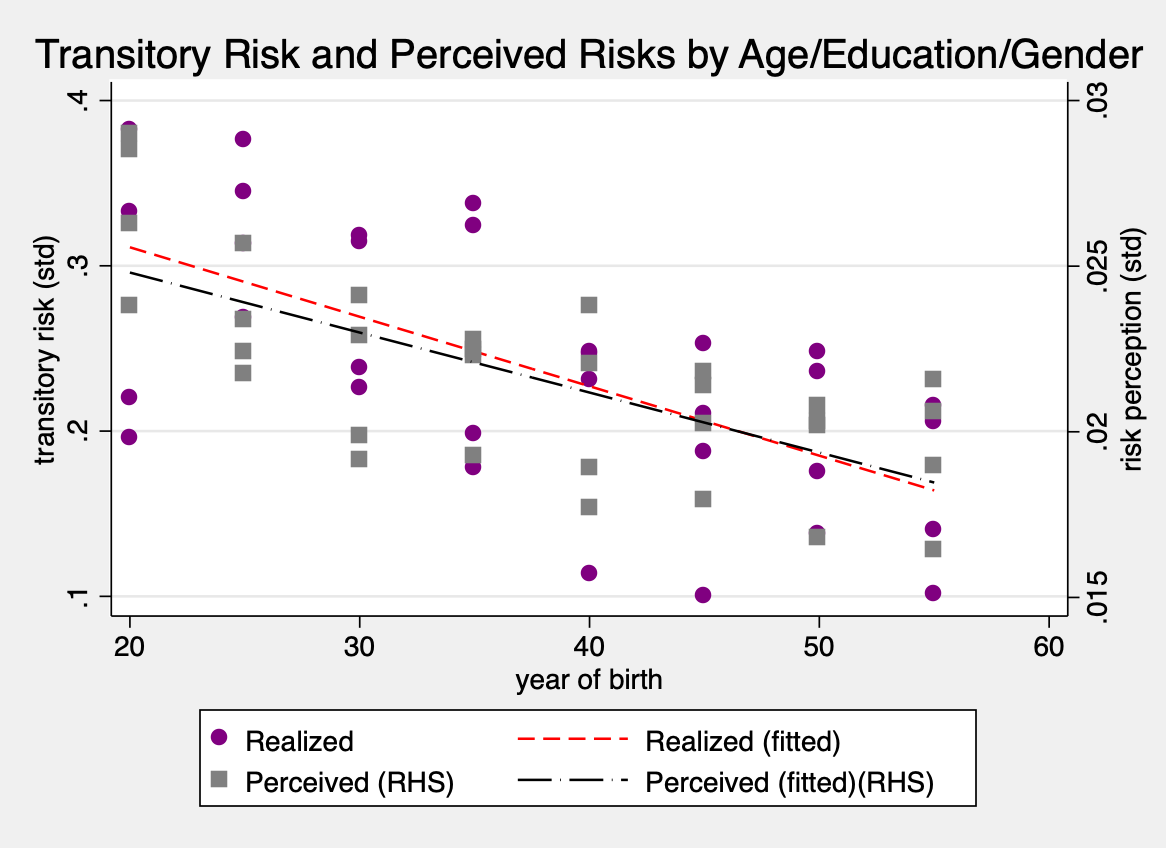
\includegraphics[width=\textwidth]{figures/log_wage_tshk_by_age_5yr_edu_gender_compare.png}
		\end{subfigure} 
	\end{figure}
	\begin{itemize}
		\item e.g. a female high school graduate aged 30-35
		\quad  \hyperlink{appendix:cohort_age_component_compare}{\beamerbutton{5-yr cohort/education/gender}}  
	\end{itemize}
	\hyperlink{monthly_decomposition_compare}{\beamerbutton{Back}} 
\end{frame}


\begin{frame}{Appendix: PR by age/education}
	\begin{figure}[ht]
		%\caption{Perceived Risk} 
		\label{appendix:age_educ_compare_figure}
		\centering
		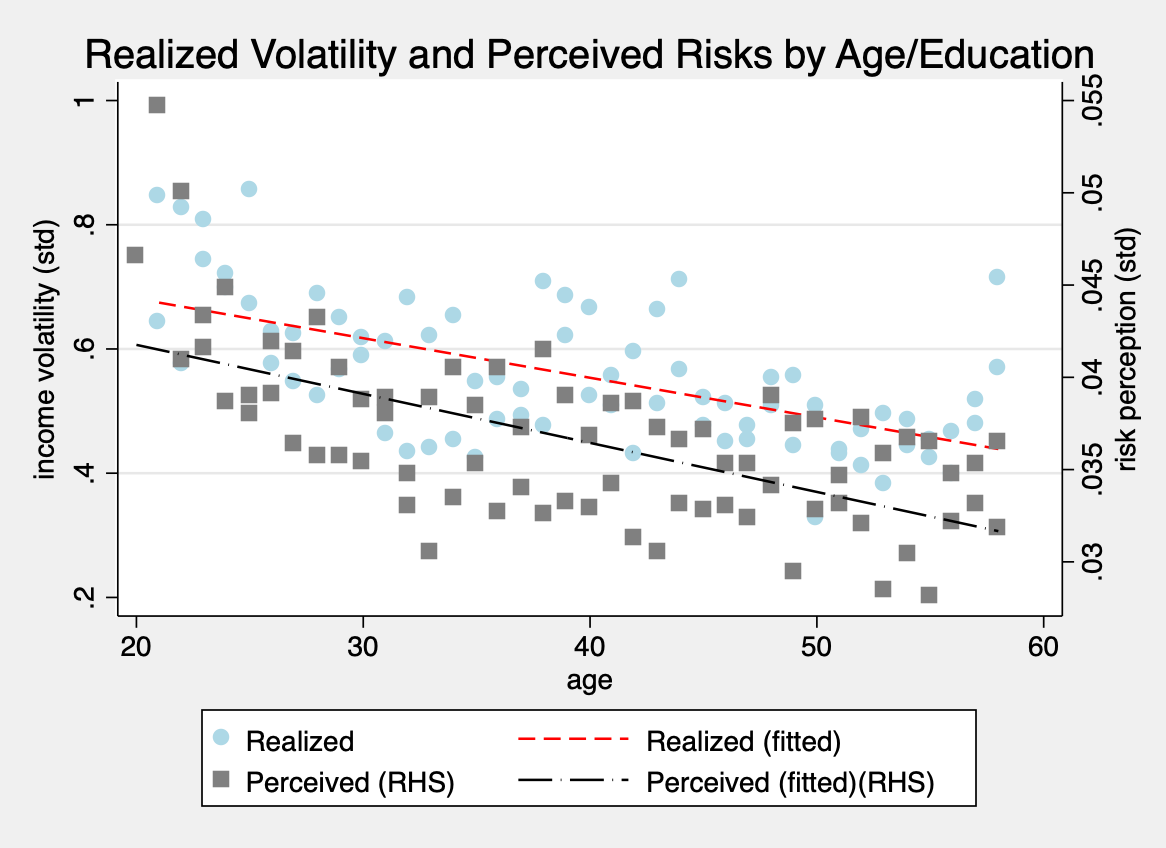
\includegraphics[width=0.7\textwidth]{figures/real_log_wage_shk_gr_by_age_edu_compare.png}
	\end{figure}
	\begin{itemize}
		\item e.g. a 35-year old high school graduate \quad  \hyperlink{age_compare}{\beamerbutton{Back}} 
		%	\item in line with existing findings, for instance  
		%	\cite{bloom2018great}. 
	\end{itemize}
\end{frame}



\begin{frame}{Appendix: PR by cohort/education/gender}
	\label{cohort_compare}
	\begin{figure}[ht]
		\label{appendix: compare_by_cohort}
		\centering
		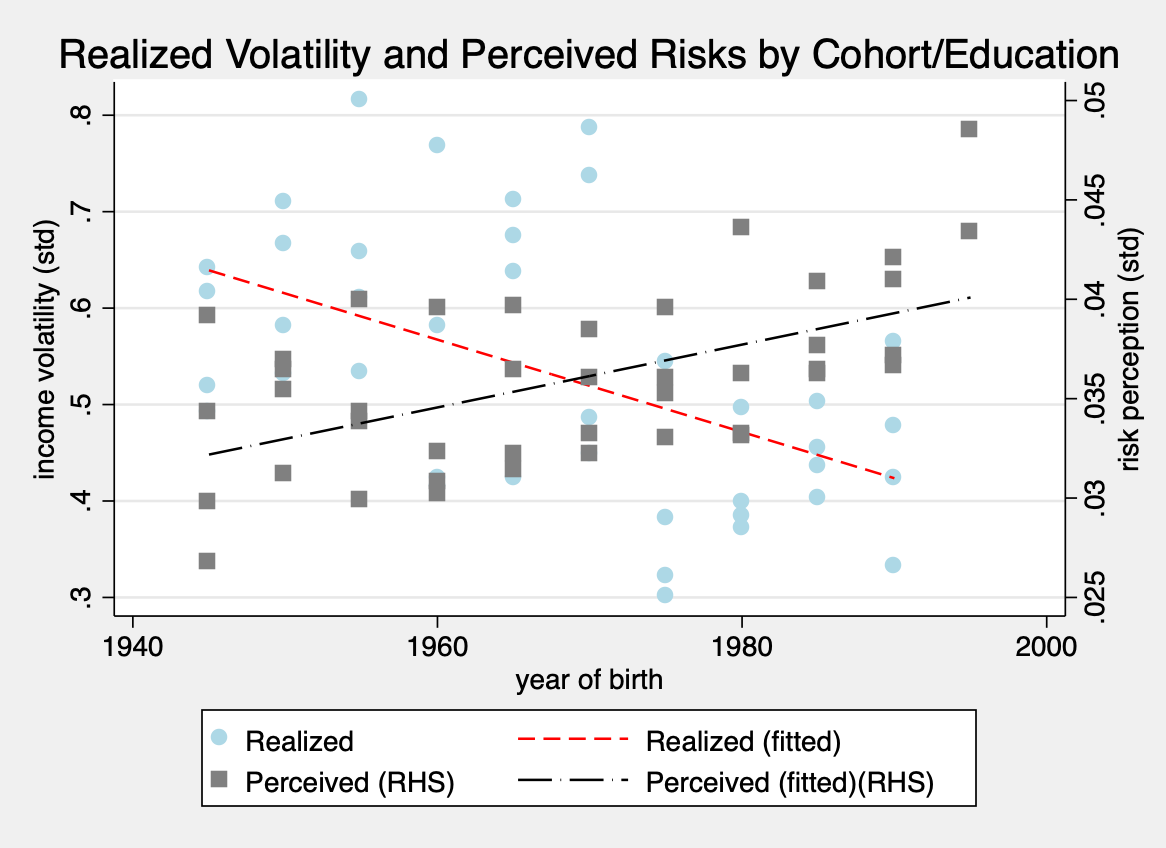
\includegraphics[width=0.6\textwidth]{figures/real_log_wage_shk_gr_by_byear_5yr_edu_gender_compare.png}
	\end{figure}
	\begin{itemize}
		\item e.g. a male higher school graduate born between 1990-1995 \quad \hyperlink{appendix:cohort_compare_figure}{\beamerbutton{inequality}}   
		\quad \hyperlink{appendix1:cohort_edu_compare_figure}{\beamerbutton{inequality by 5-year/education}}   
		\quad \hyperlink{appendix2:cohort_edu_compare_figure}{\beamerbutton{5-year/education}}     \quad  \hyperlink{age_compare}{\beamerbutton{Back}} 
		\item declining income volatlity between 1978-2013 \cite{sabelhaus2010great}, \cite{bloom2018great} 
	\end{itemize}
\end{frame}

\begin{frame}{Appendix: PR by cohort}
	\begin{figure}[ht]
		%\caption{Perceived Risk} 
		\label{appendix:cohort_compare_figure}
		\centering
		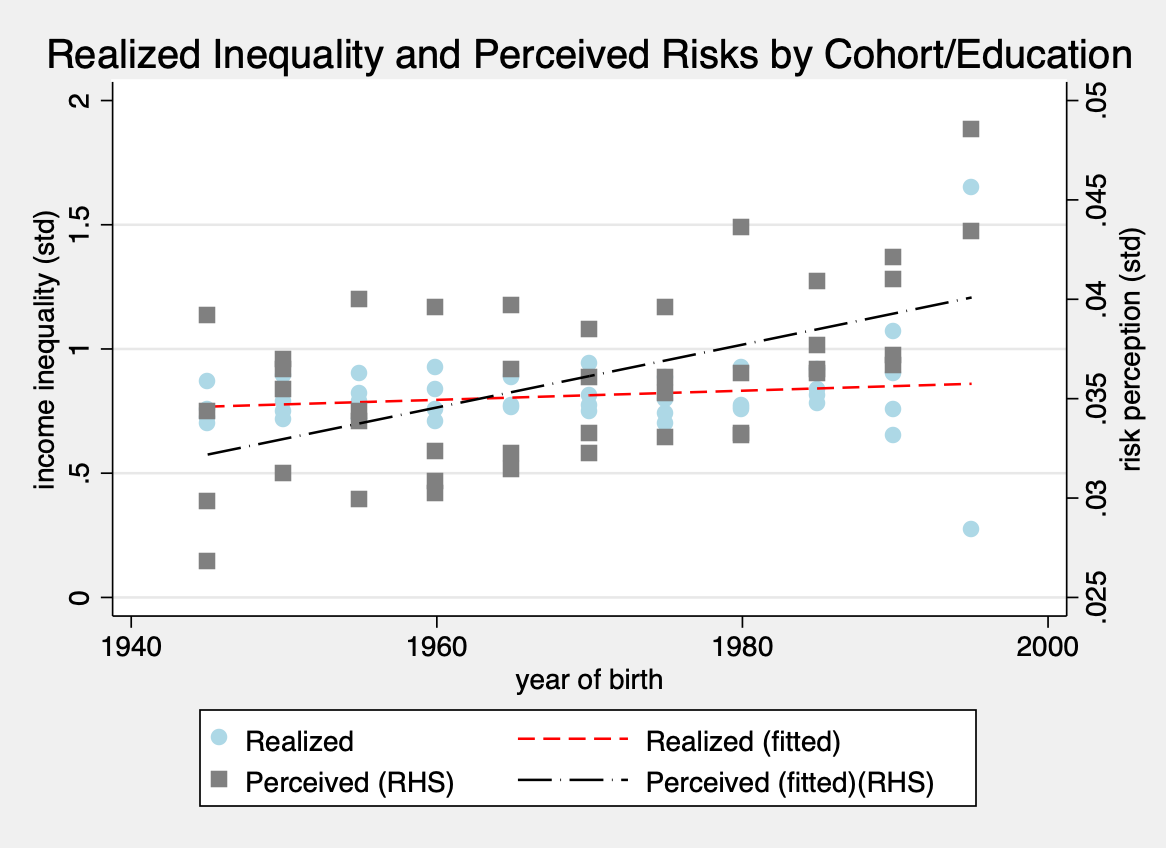
\includegraphics[width=0.7\textwidth]{figures/real_log_wage_shk_by_byear_5yr_edu_gender_compare.png}
	\end{figure}
	\begin{itemize}
		\item e.g. a female college graduate born between 1970-1975   \quad  \hyperlink{cohort_compare}{\beamerbutton{Back}} 
		%	\item in line with existing findings, for instance  
		%	\cite{bloom2018great}. 
	\end{itemize}
\end{frame}


\begin{frame}{Appendix: PR by cohort/education}
	\begin{figure}[ht]
		%\caption{Perceived Risk} 
		\label{appendix1:cohort_edu_compare_figure}
		\centering
		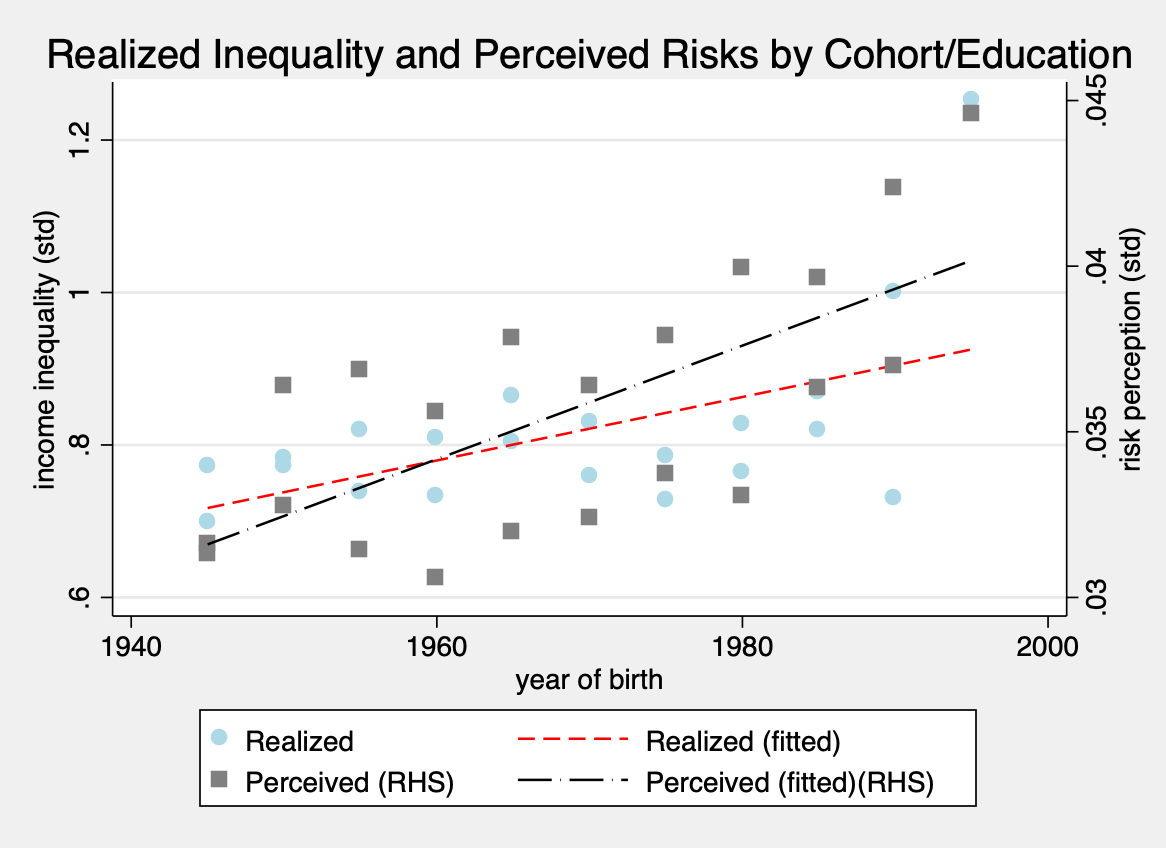
\includegraphics[width=0.7\textwidth]{figures/real_log_wage_shk_by_byear_5yr_edu_compare.png}
	\end{figure}
	\begin{itemize}
		\item e.g. a high school graduate born between 1985-1990  \quad  \hyperlink{cohort_compare}{\beamerbutton{Back}} 
		%	\item in line with existing findings, for instance  
		%	\cite{bloom2018great}. 
	\end{itemize}
\end{frame}


\begin{frame}{Appendix: PR by cohort/education}
	\begin{figure}[ht]
		%\caption{Perceived Risk} 
		\label{appendix2:cohort_edu_compare_figure}
		\centering
		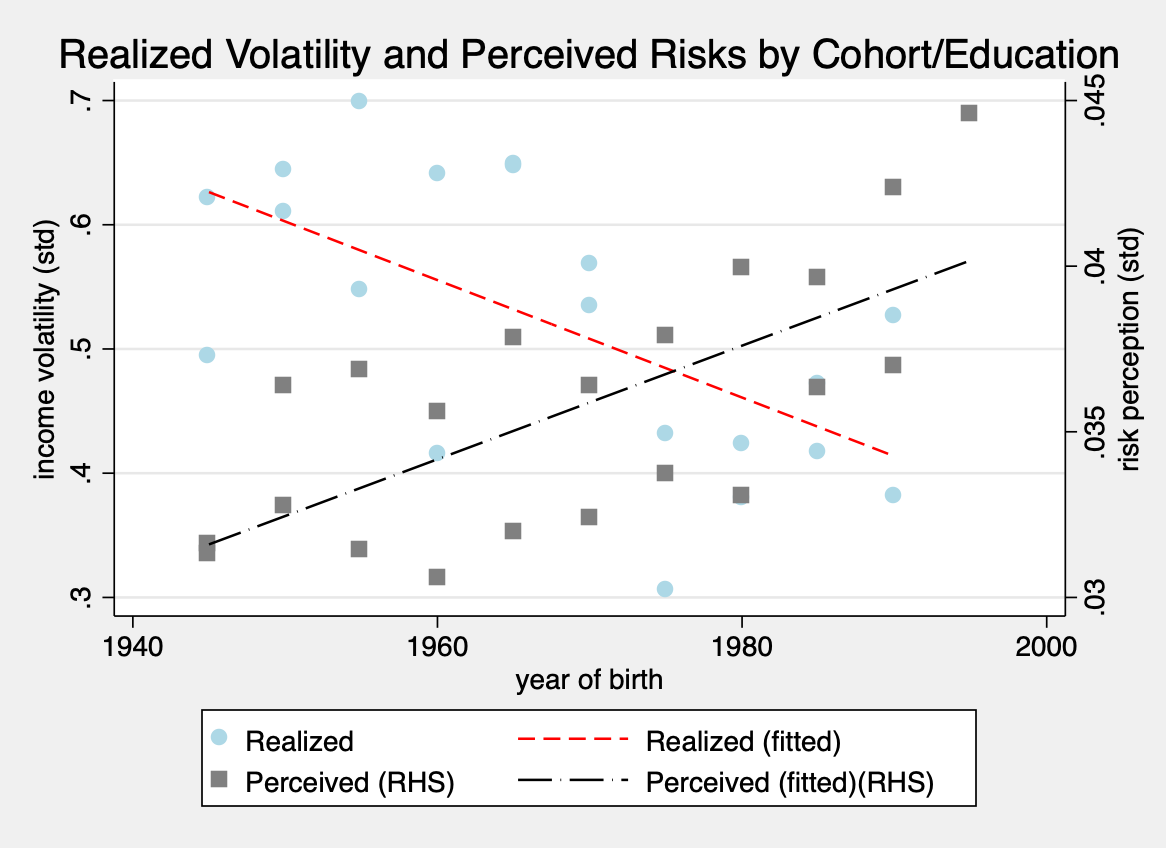
\includegraphics[width=0.7\textwidth]{figures/real_log_wage_shk_gr_by_byear_5yr_edu_compare.png}
	\end{figure}
	\begin{itemize}
		\item a college graduate born between 1985-1990  \quad  \hyperlink{cohort_compare}{\beamerbutton{Back}} 
		%	\item in line with existing findings, for instance  
		%	\cite{bloom2018great}. 
	\end{itemize}
\end{frame}



\begin{frame}{Appendix: expected income growth and recent (past) wage growth}
	\label{appendix:tsMean3mvrexp_he}
	\begin{itemize}
		\item $\overline{\text{exp}_{t}} $: average expected growth across individuals
		\item  quarterly growth in average hourly wage
	\end{itemize}
	\begin{figure}
		\centering
		\label{ts_exp}
		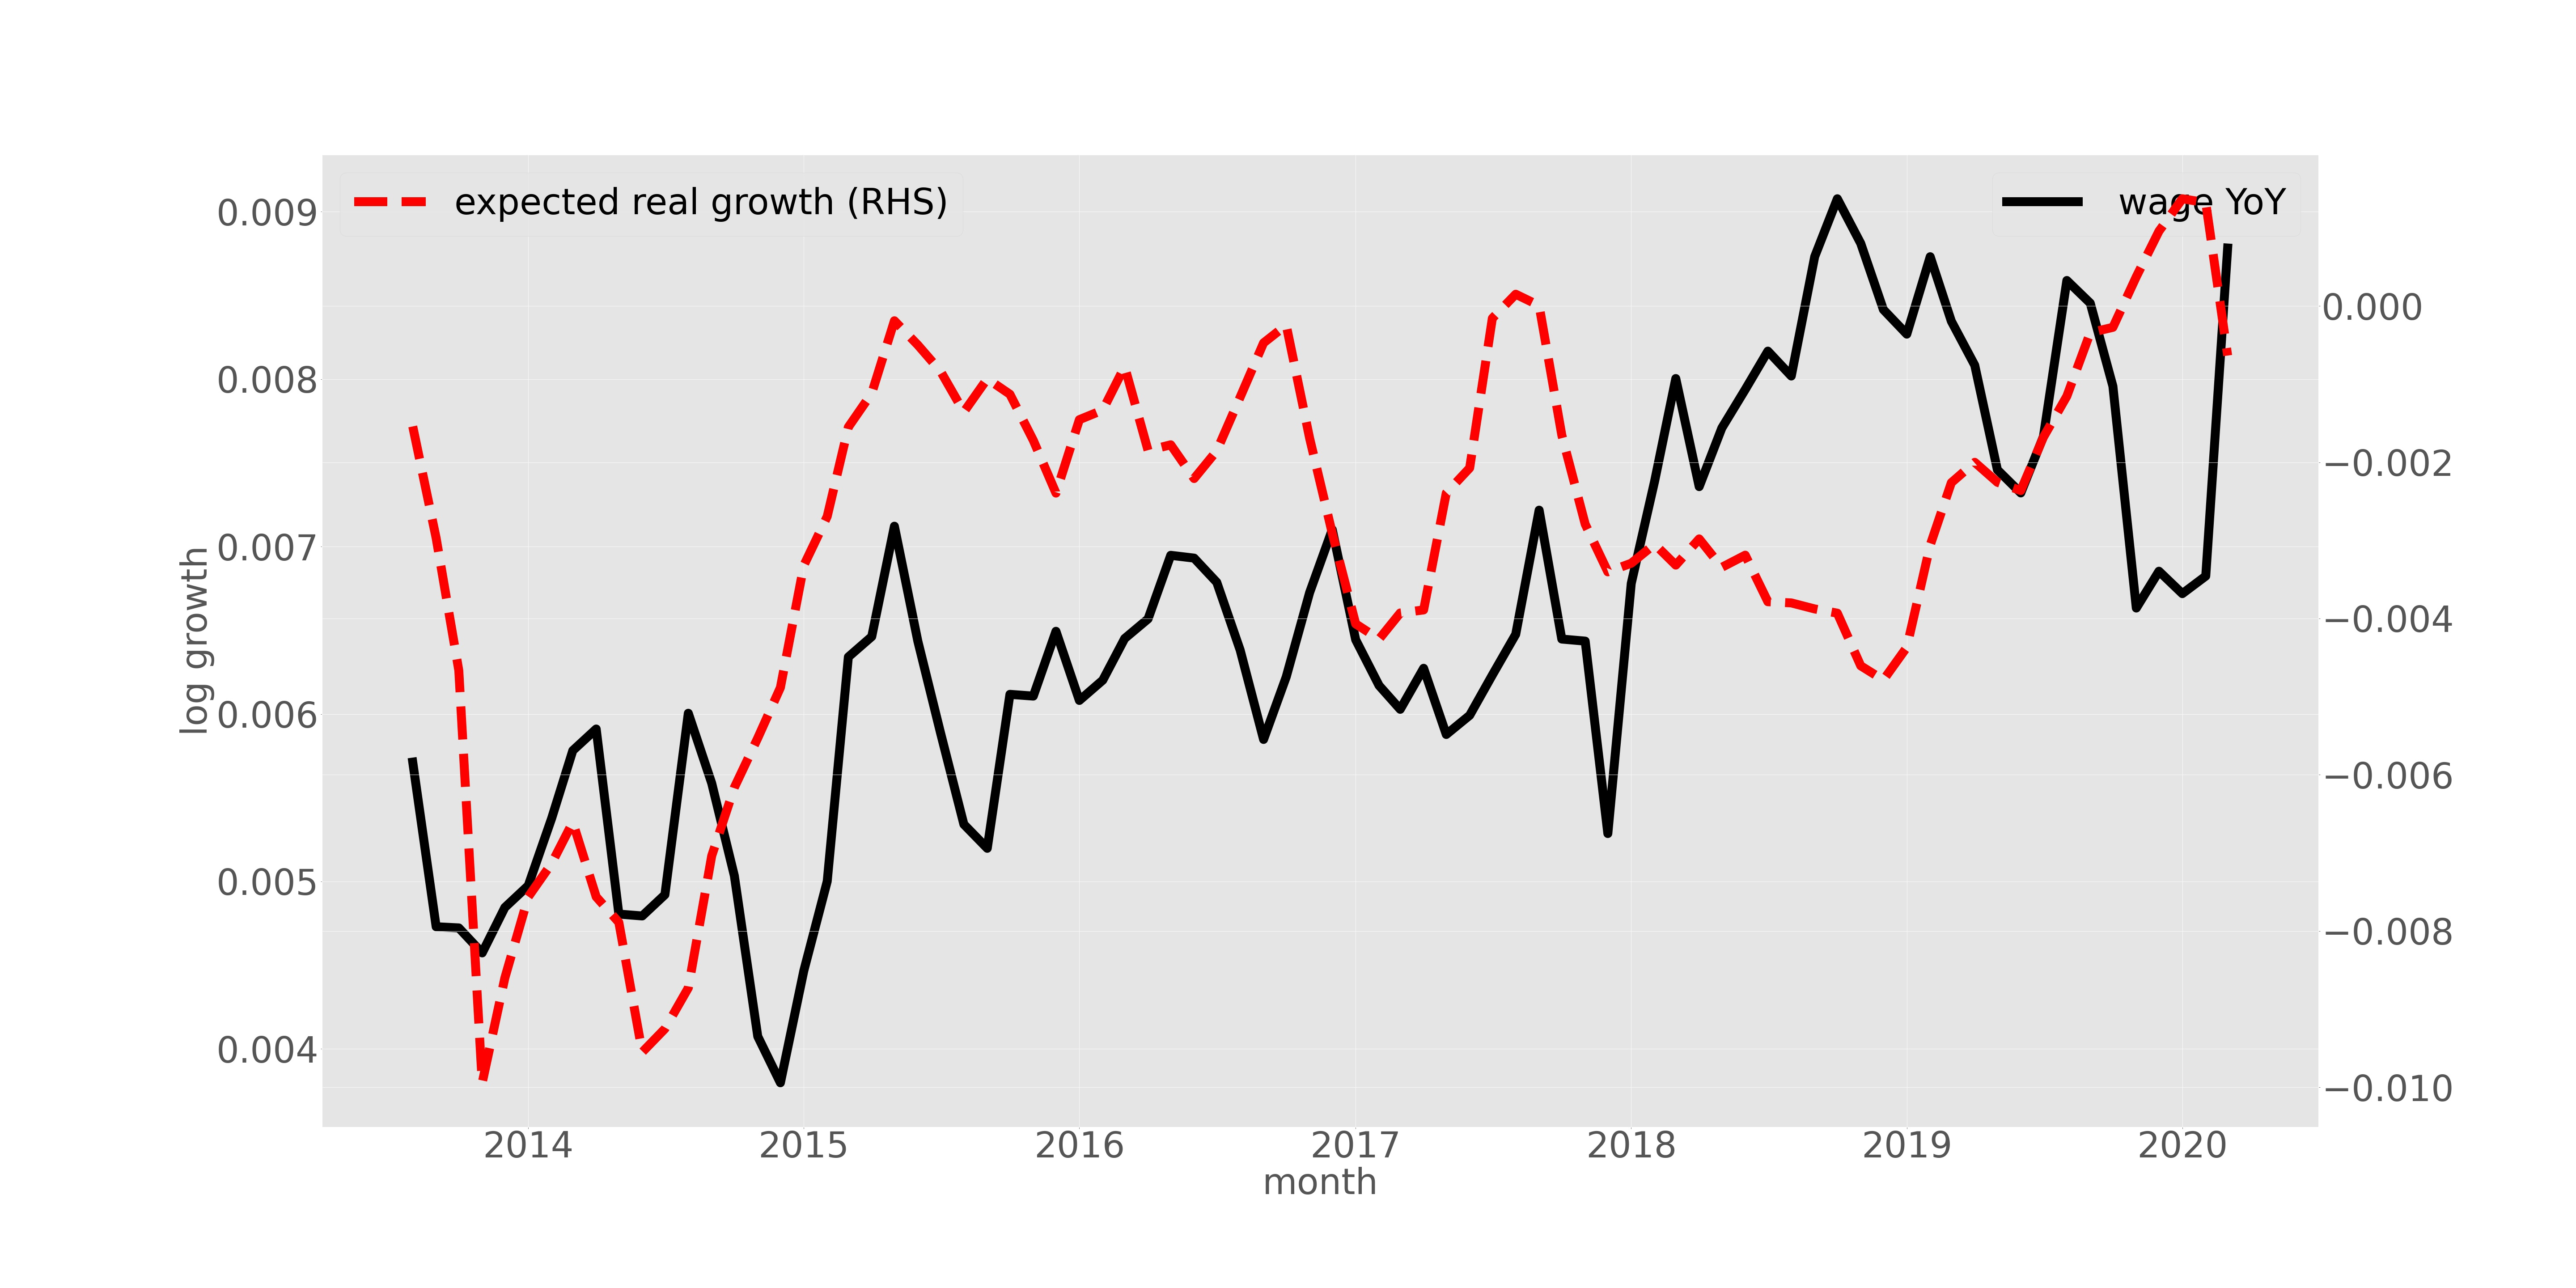
\includegraphics[width=0.9\textwidth]{figures/tsMean3mvrexp_he.jpg}
	\end{figure}
	\quad  \hyperlink{tsMean3mvrvar_he}{\beamerbutton{Back}} 
\end{frame}


\begin{frame}{Appendix: by \textbf{5-yr of birth/age}}
	\label{appendix:cohort_age_compare}
	\begin{figure}[ht]
		%\caption{Perceived Risk} 
		\centering
		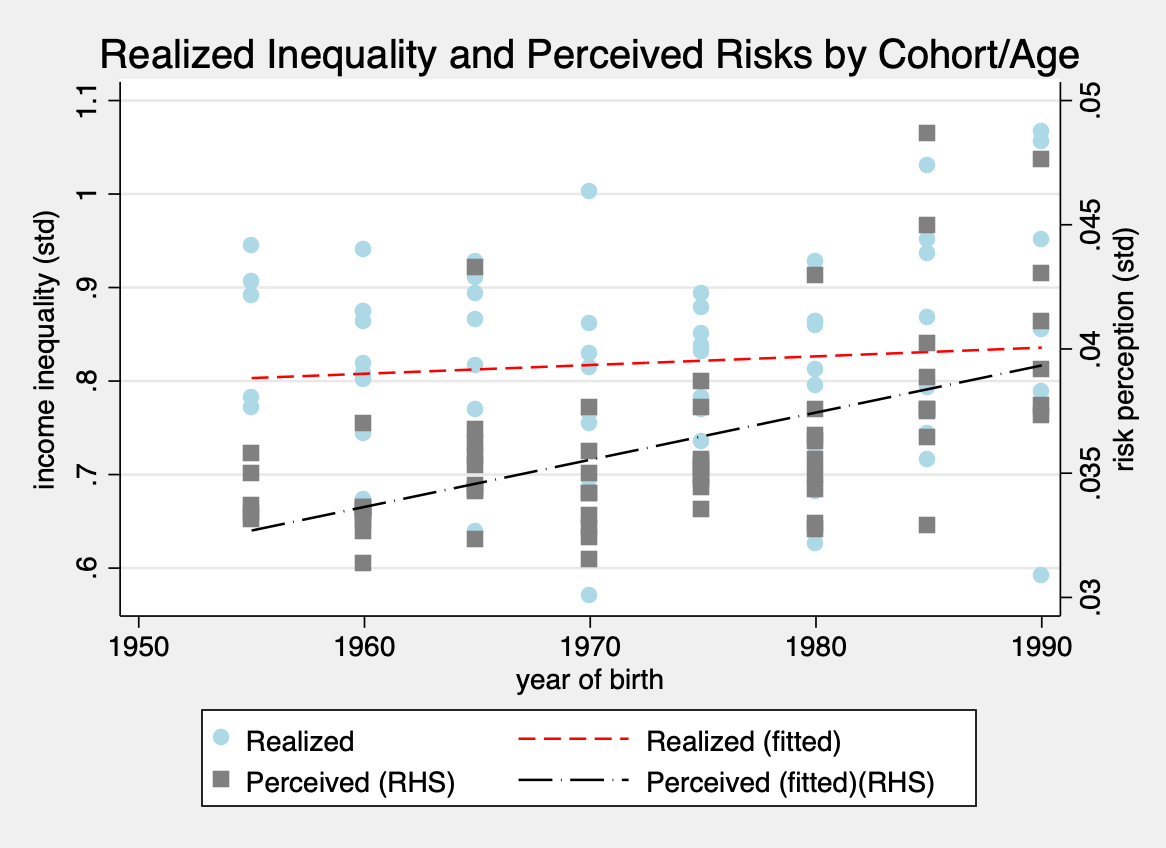
\includegraphics[width=0.65\textwidth]{figures/real_log_wage_shk_by_byear_age_compare.png}
		%	\begin{subfigure}[b]{0.46\textwidth}
		%			\caption{skewness}
		%			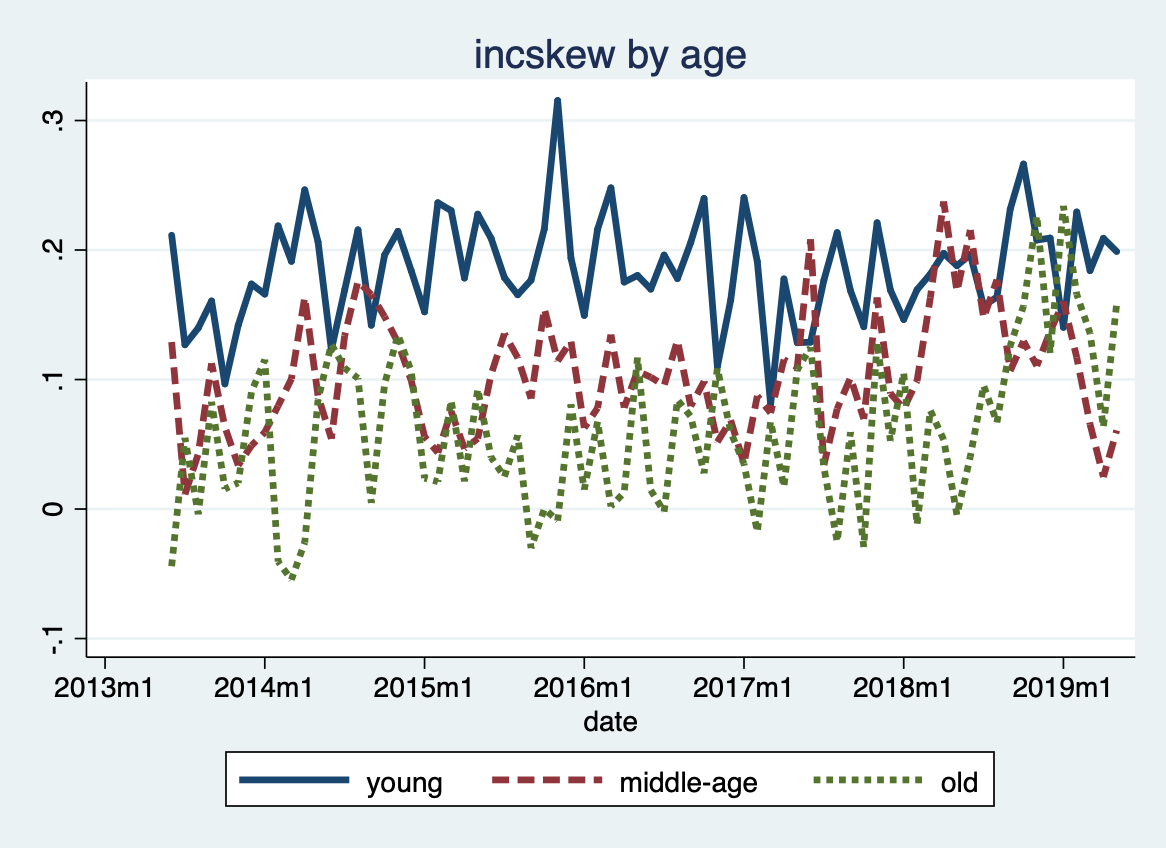
\includegraphics[width=\textwidth, height = 0.33\textheight]{figures/ts_incskew_age_g_mean.png}
		%	\end{subfigure}
	\end{figure}
	\begin{itemize}
		\item e.g. a 25-year old born between 1985-1990
		\item only possible for post-2013 sample 
		\quad \hyperlink{cohort_age_compare}{\beamerbutton{Back}}     
	\end{itemize}
\end{frame}

\begin{frame}{Appendix: permanent versus transitory risks}
	\label{appendix:cohort_age_component_compare}
	\begin{figure}[ht]
		%\caption{Perceived Risk} 
		\centering
		\begin{subfigure}[b]{0.44\textwidth}
			\caption{permanent}
			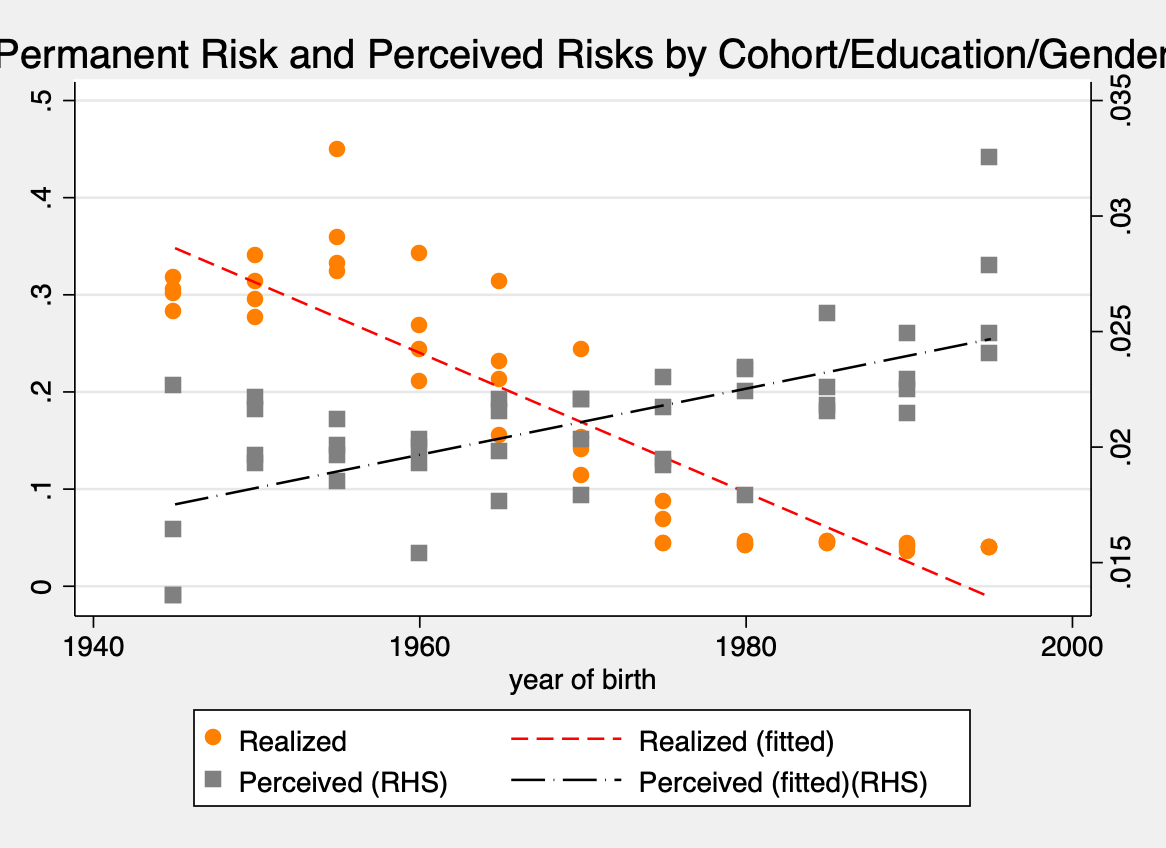
\includegraphics[width=\textwidth]{figures/log_wage_pshk_by_byear_5yr_edu_gender_compare.png}
		\end{subfigure}
		\begin{subfigure}[b]{0.44\textwidth}
			\caption{transitory}
			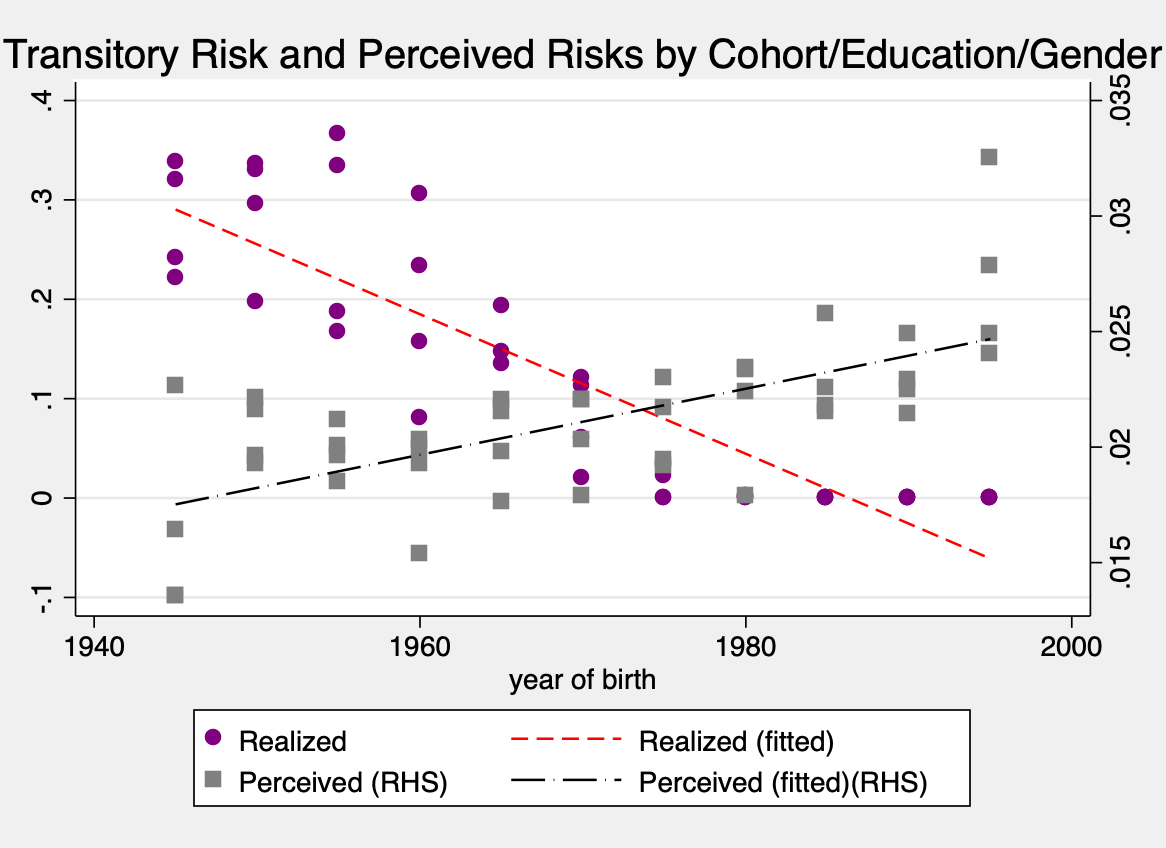
\includegraphics[width=\textwidth]{figures/log_wage_tshk_by_byear_5yr_edu_gender_compare.png}
		\end{subfigure} 
	\end{figure}
	\begin{itemize}
		\item e.g. a female high school graduate born between 1985-1990
		\quad  \hyperlink{cohort_age_component_compare}{\beamerbutton{Back}}  
	\end{itemize}
\end{frame}



\begin{frame}{Appendix: monthly earning inequality and volatility}
	\label{appendix:monthly_inequality_vol}
	\begin{figure}[ht]
	\centering
	\begin{subfigure}[b]{0.46\textwidth}
		\caption{Inequality}
		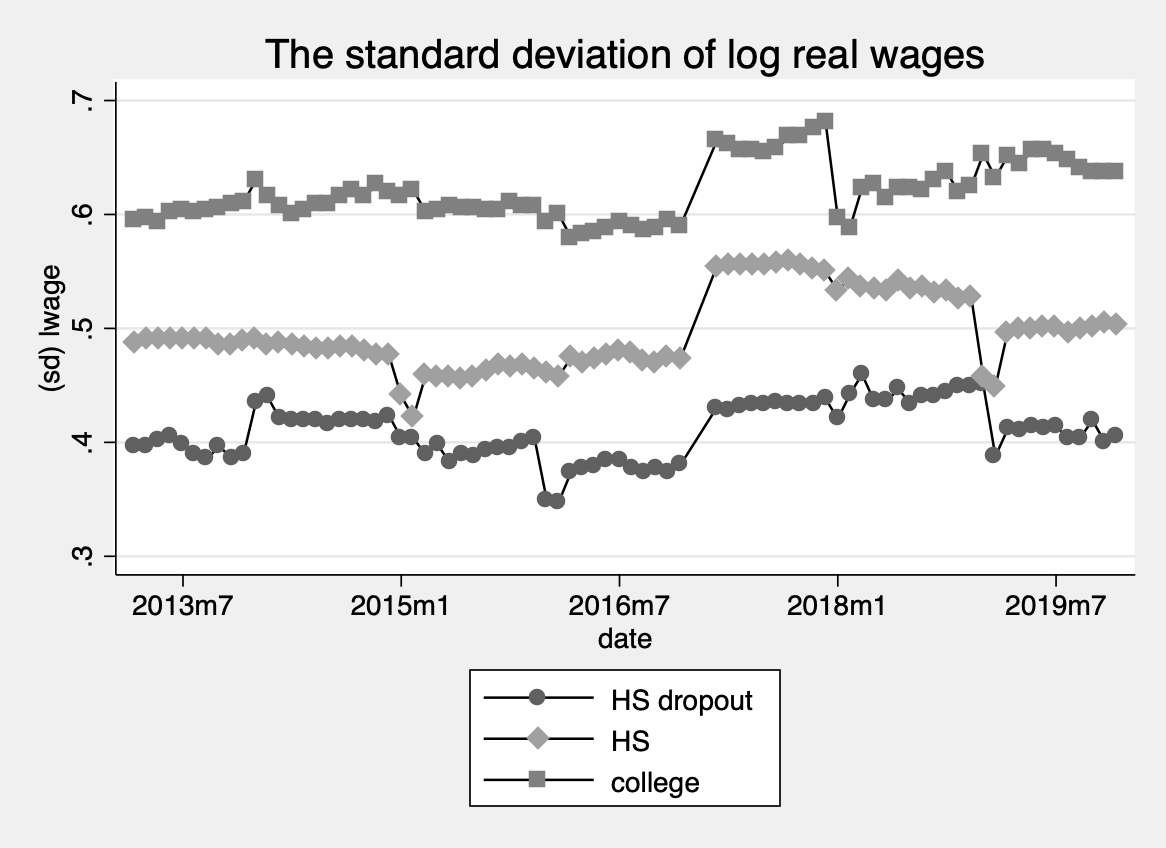
\includegraphics[width=\textwidth]{figures/log_wage_sd_by_edu.png}
	\end{subfigure}
	\begin{subfigure}[b]{0.46\textwidth}
		\caption{Volatility}
		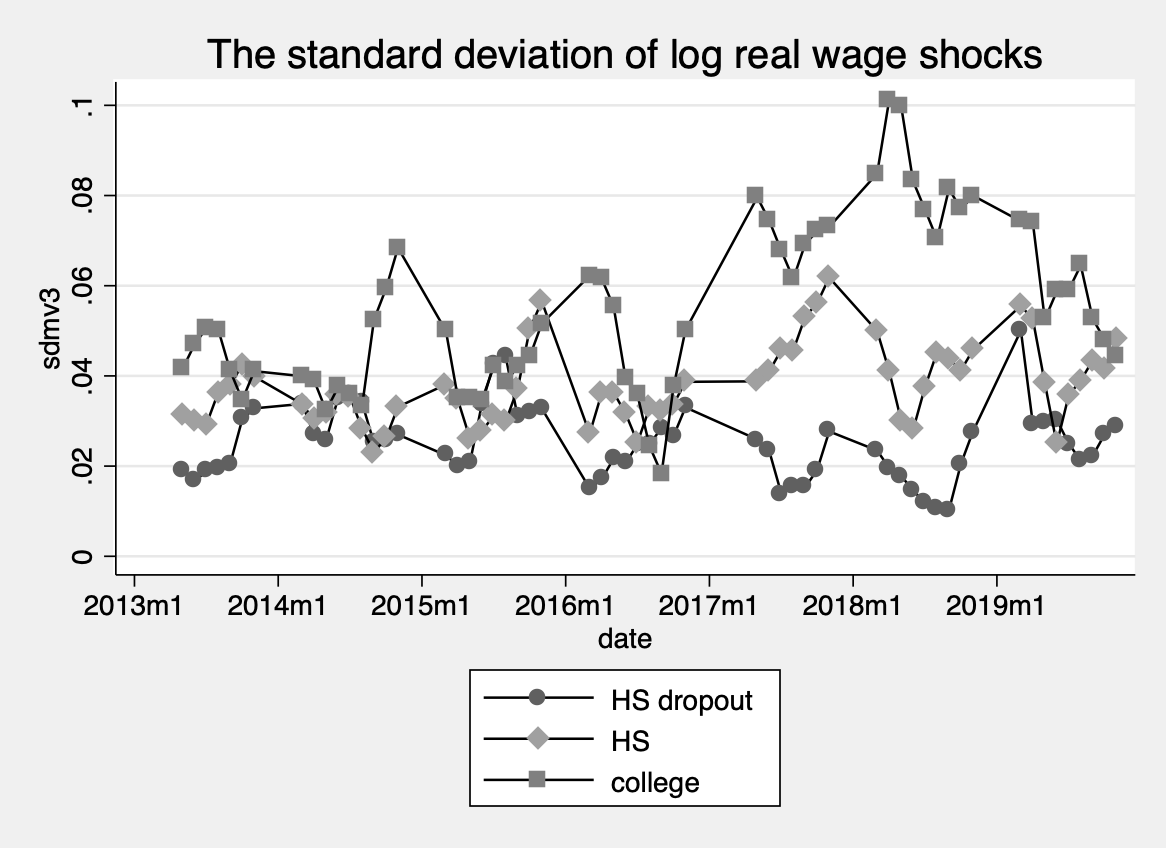
\includegraphics[width=\textwidth]{figures/log_wage_shk_gr_sd_by_edu.png}
	\end{subfigure} 
\end{figure}
	\hyperlink{monthly_decomposition_compare}{\beamerbutton{Back}} 
\end{frame}

\begin{frame}{Appendix: estimation of subjective risk profile}
	\label{appendix:RegimeEstimationDetail}
	
	\begin{equation*}
		\begin{split}
				\log(\tilde {\text{var}}_{i,t})= (12+\frac{1}{12\kappa^2})\tilde \sigma^2_{i,t,\psi} + \xi_{t}+\eta_{i}+ \epsilon_{i,t}
			\end{split}
	\end{equation*}
	\begin{itemize}
		
		\item $\kappa$: externally assumed ratio of permanent and transitory risks $\frac{\tilde \sigma_{i,t,\psi}}{\tilde \sigma_{i,t,\theta}}$
		\end{itemize}
	\hyperlink{RegimeEstimation}{\beamerbutton{Back}} 
\end{frame}


\bibliographystyle{apalike}
\bibliography{PerceivedIncomeRisk}


\end{document}
